\documentclass{article}
\usepackage{graphicx} % Required for inserting images

\title{Digital Control Systems Coursework: Omar Ben-Gacem}
\author{Omar Ben-Gacem}
\date{January 2025}



%%%%%%%%%%%%     Formatting     %%%%%%%%%%%%

\usepackage[sorting=none]{biblatex} %Imports biblatex package

\addbibresource{bibliography.bib} %Import the bibliography file
\usepackage[margin=1in,headsep=.5in]{geometry}
\usepackage{amsmath} % for bmatrix and pmatrix
\usepackage{amssymb}
\usepackage{wrapfig}
\usepackage{caption}
\usepackage{fancyhdr}
\usepackage{subcaption}
\usepackage{gensymb}
\usepackage{float}
\usepackage{ragged2e}
\usepackage{booktabs} % For better table formatting
\usepackage[export]{adjustbox}
\geometry{
 a4paper,
 total={170mm,257mm},
 left=19mm,
 right=19mm,
 top=23mm,
 bottom=23mm
 }
\renewcommand{\sectionmark}[1]{%
    \markright{\MakeUppercase{#1}}%
}



\title{Digital Control Systems Coursework Submission}
\author{Omar Ben-Gacem}
\pagestyle{fancy}
\fancyhead[RO]{{\rightmark}}
\date{November 2024}
\lhead{Omar Ben-Gacem\\01883771\\Digital Control Systems Coursework}






%%%%%%%%%%%%     Formatting     %%%%%%%%%%%%


\begin{document}


% \section*{Executive Summary}
% \begin{equation}
R = \left(\begin{array}{cccc} 0 & \frac{1}{M} & -\frac{F}{M^2} & \frac{F^2}{M^3}\\ \frac{1}{M} & -\frac{F}{M^2} & \frac{F^2}{M^3} & -\frac{F^3}{M^4}\\ 0 & -\frac{1}{L\,M} & \frac{F}{L\,M^2} & -\frac{g}{L^2\,M}-\frac{F^2}{L\,M^3}\\ -\frac{1}{L\,M} & \frac{F}{L\,M^2} & -\frac{g}{L^2\,M}-\frac{F^2}{L\,M^3} & \frac{\frac{F^3}{L\,M^3}+\frac{F\,g}{L^2\,M}}{M} \end{array}\right)
\end{equation}



\section{System Dynamics (Part A)}
The system being modeled is an inverted pendulum attached to a sliding cart. The objective is to control the linear displacement of the cart in order to hold the pendulum in an inverted position ($\phi=0$). Equation \ref{eqofm} gives the Newtonian equations of motion for the cart-pendulum system.

\[
\begin{cases}
  M \ddot{s}(t) + F \dot{s}(t) - \mu(t) & = 0 \\
    \ddot{\phi}(t) - \frac{g}{L} \ddot{s}(t) \sin({\phi}(t)) - \frac{\mu(t)}{L} \cos(\phi(t)) & = 0
\end{cases}
\]

\subsection*{A1) Standard Form}
To write the cart-pendulum system in standard form, the state variable $\underline{x}$ and the input $\underline{u}$ must be identified. The applied force $\mu(t)$ acts as the only input to this system. By inspection of the equations of motion, it is trivial to show that displacement $s$ and angle $\phi$ both have first- and second-order differential terms, thus making state variable $\underline{x} = [s, \dot s, \phi, \dot\phi]^T$. Equation \ref{eqofm} can be rearranged and reduced to give Equation \ref{fofx} which acts as the state update function.

\begin{equation}\label{fofx}
    \dot{x}=\begin{bmatrix}\dot{s} \\ \ddot{s} \\ \dot{\phi} \\ \ddot{\phi}\end{bmatrix} = f(\underline{x},\underline{u}) = \n\left(\begin{array}{cccc} 0 & 1 & 0 & 0\\ 0 & -\frac{F}{M} & 0 & 0\\ 0 & 0 & 0 & 1\\ 0 & \frac{F}{LM} & \frac{g}{L} & 0 \end{array}\right)
\n \begin{bmatrix} s \\ \dot{s} \\ \phi \\ \dot{\phi}\end{bmatrix} +     \begin{bmatrix}
        0 \\
        \frac{1}{M} \\
        0 \\
        -\frac{1}{L M}
    \end{bmatrix}\,\mu(t)
\end{equation}

\subsection*{A2) Free Response Equilibrium}
Setting $u=\mu(t)=0$ gives the free response of the system, where the equilibrium of this system are values of $\underline{\dot x}=\underline{0}$. The values of $\underline{x}$ that satisfy this criteria are shown below in Equation \ref{ueqzero}.

\begin{equation}\label{ueqzero}
\begin{bmatrix}
    \dot s \\ \ddot s \\ \dot \phi \\ \ddot \phi
\end{bmatrix} =  \begin{bmatrix}
    0 \\ 0 \\ 0 \\ 0
\end{bmatrix} = \begin{bmatrix}
    \dot{s} \\
    \frac{u}{M}-\frac{F\dot{s}}{M}  \\
    \dot{\phi} \\
     \frac{g\sin\left(\phi \right)}{L}-\frac{u\cos\left(\phi \right)}{LM}+\frac{F\dot{s}\cos\left(\phi \right)}{LM} \\
\end{bmatrix} \rightarrow \mu=0 \rightarrow \underline{x} = \begin{bmatrix}
    s \\ \dot s \\ \phi \\ \dot \phi
\end{bmatrix} = \begin{bmatrix}
    \Re \\
    0 \\
    \pi n, n \in \mathbb{Z} \\
    0 \\
\end{bmatrix}
\end{equation}



Equation \ref{fofx} shows that the displacement of the cart, $s$, has no impact on the systems ability to reach equilibrium. Thus the possible values of $s$ is determined to be the set of real numbers. In practice, it is bounded to be a reasonable amount of translational motion. The values of $\phi$ is set to be any period of $\pi$, meaning the pendulum is either vertically up or down. 

\subsection*{A3) Linearization About an Equilibrium}
Given a point to linearize about, the state space model of the non-linear system $f(\underline{x},\underline{u})$ can be derived using the Jacobian operator to give the Jacobian matrix. The linearization should yield an equation of the form $\dot x = Ax+Bu$. Equation \ref{jacobian} shows the taking of the Jacobian vector at the point $\underline{x}=\underline{0}$, to get the matrix $A$.

\begin{equation} \label{jacobian}
    A=  \left. J\{f(\underline{x},\underline{u})\} \right|_{\underline{x}=\underline{0}} =
    \left. \begin{bmatrix}
    \frac{\partial f_1(x,u)}{\partial x_1} & \frac{\partial f_1(x,u)}{\partial x_2} & \frac{\partial f_1(x,u)}{\partial x_3} & \frac{\partial f_1(x,u)}{\partial x_4} \\
    \frac{\partial f_2(x,u)}{\partial x_1} & \frac{\partial f_2(x,u)}{\partial x_2} & \frac{\partial f_2(x,u)}{\partial x_3} & \frac{\partial f_2(x,u)}{\partial x_4} \\
    \frac{\partial f_3(x,u)}{\partial x_1} & \frac{\partial f_3(x,u)}{\partial x_2} & \frac{\partial f_3(x,u)}{\partial x_3} & \frac{\partial f_3(x,u)}{\partial x_4} \\
    \frac{\partial f_4(x,u)}{\partial x_1} & \frac{\partial f_4(x,u)}{\partial x_2} & \frac{\partial f_4(x,u)}{\partial x_3} & \frac{\partial f_4(x,u)}{\partial x_4}
    \end{bmatrix} \right|_{\underline{x}=\underline{0}}
    = \n\left(\begin{array}{cccc} 0 & 1 & 0 & 0\\ 0 & -\frac{F}{M} & 0 & 0\\ 0 & 0 & 0 & 1\\ 0 & \frac{F}{LM} & \frac{g}{L} & 0 \end{array}\right)
\n
\end{equation}


To find matrix $B$, the Jacobian is taken again, however, this time with respect to input $u$. Equation \ref{jB} shows the derivation of the input Jacobian for equilibrium $\underline{x}=\underline{0}$.

\begin{equation} \label{jB}
    B=  \left. \frac{\partial f(\underline{x},\underline{u})}{\partial \underline{u}} \right|_{\underline{x}=\underline{0}} =
    \left. \begin{bmatrix}
    \frac{\partial f_1(x,u)}{\partial u} \\
    \frac{\partial f_2(x,u)}{\partial u} \\
    \frac{\partial f_3(x,u)}{\partial u} \\
    \frac{\partial f_4(x,u)}{\partial u}
    \end{bmatrix} \right|_{\underline{x}=\underline{0}}
    =     \begin{bmatrix}
        0 \\
        \frac{1}{M} \\
        0 \\
        -\frac{1}{L M}
    \end{bmatrix}
\end{equation}



This can be put into full state space representation as shown in Equation \ref{linized}. This gives the full state-space representation of the cart-pendulum system, and can be used to describe the local behavior of the system. about the point the equilibrium was taken.
\begin{equation}\label{linized}
    \underline{\dot{x}} = \begin{bmatrix} \dot{s} \\ \ddot{s} \\ \dot{\phi} \\ \ddot{\phi} \end{bmatrix} =\n\left(\begin{array}{cccc} 0 & 1 & 0 & 0\\ 0 & -\frac{F}{M} & 0 & 0\\ 0 & 0 & 0 & 1\\ 0 & \frac{F}{LM} & \frac{g}{L} & 0 \end{array}\right)
\n\begin{bmatrix} s \\ \dot{s} \\ \phi \\ \dot{\phi} \end{bmatrix}+     \begin{bmatrix}
        0 \\
        \frac{1}{M} \\
        0 \\
        -\frac{1}{L M}
    \end{bmatrix} [\mu]
\end{equation}

\subsection*{A4) Linear Dynamics}
The system has output function of the states, but not their velocities.This means that output $\underline{y}(t)=[s(t), \phi(t)]^T$. To achieve this, output equation $\underline{y}(t)=C\underline{x}+D\underline{u}$. It is trivial to show that $D$ is the zero vector, and C is a $2\times4$ vector with  the value $1$ in position $C_{1,1}$ and $C_{2,3}$, and the rest being zero. This gives the linear dynamics state space representation as shown in Equation \ref{lindy}

\begin{equation}\label{lindy}
    \begin{bmatrix}
        \underline{\dot x}(t) \\ \underline{y}(t)
    \end{bmatrix} = \begin{bmatrix}
        A & B \\ C & D
    \end{bmatrix}\begin{bmatrix}
        \underline{x}(t) \\ \underline{u}(t)
    \end{bmatrix} = \n\left(\begin{array}{ccccc} 0 & 1 & 0 & 0 & 0\\ 0 & -\frac{F}{M} & 0 & 0 & \frac{1}{M}\\ 0 & 0 & 0 & 1 & 0\\ 0 & \frac{F}{LM} & \frac{g}{L} & 0 & -\frac{1}{LM}\\ 1 & 0 & 0 & 0 & 0\\ 0 & 0 & 1 & 0 & 0 \end{array}\right)
\n\begin{bmatrix}
        \underline{x}(t) \\ \underline{u}(t)
    \end{bmatrix}
\end{equation}

\subsection*{A5) Reachability}
The reachability matrix is used to determine if all possible states are reachable given the dynamics of the system. If the reachability matrix is full rank, then it can be determined that the system has a possible feedback loop that can stabilize it. Equation \ref{reach} shows the reachability matrix, that was derived using the matrices found in Equations \ref{jacobian} and \ref{jB}.

\begin{equation}\label{reach}
    R =
    \begin{bmatrix}
        B & AB & A^2B & A^3B
    \end{bmatrix}
    =\begin{equation}
R = \left(\begin{array}{cccc} 0 & \frac{1}{M} & -\frac{F}{M^2} & \frac{F^2}{M^3}\\ \frac{1}{M} & -\frac{F}{M^2} & \frac{F^2}{M^3} & -\frac{F^3}{M^4}\\ 0 & -\frac{1}{L\,M} & \frac{F}{L\,M^2} & -\frac{g}{L^2\,M}-\frac{F^2}{L\,M^3}\\ -\frac{1}{L\,M} & \frac{F}{L\,M^2} & -\frac{g}{L^2\,M}-\frac{F^2}{L\,M^3} & \frac{\frac{F^3}{L\,M^3}+\frac{F\,g}{L^2\,M}}{M} \end{array}\right)
\end{equation}

\end{equation}

It is trivial to see that this matrix is full rank, however to confirm, the determinant of the reachability matrix can be shown to be $det(R)=\frac{g^2}{L^4M^4}$. Thus for any non-zero gravity, pendulum length, or cart mass, this system will be full rank, and thus reachable.

\subsection*{A6) Observability}
Similarly to the reachability matrix, the observability matrix gives insight into if the system's ability to identify it's own state for use in feedback. Equation \ref{obsv} shows the observability matrix and it's definition. Without proof, it can be trivially shown that this is a full rank matrix, making the cart-pendulum system fully observable.
\begin{equation}\label{obsv}
    O=\begin{bmatrix}
        C \\ CA
    \end{bmatrix} = \begin{bmatrix}
1 & 1 & 1 & 1 \\
0 & 0 & 0 & 0 \\
0 & 0 & 0 & 0 \\
0 & 0 & 0 & 0
\end{bmatrix}

\end{equation}


\section{Computational Simulations (Part B)}


\subsection*{B1) Linear Time Feedback Controller}
A full state feedback controller of the form $u=Kx$ was designed to control the system back to the state $\underline{x}=\underline{0}$. With this specific controller configuration, the state update equation can be simplified to the below expression.

\begin{equation}\label{new_state_eq}
    \dot x = Ax+Bu = Ax+B(Kx) = (A+BK)x   \Rightarrow   x(t)=e^{A+BK}x(0)
\end{equation}
\newline

Equation \ref{new_state_eq} is solved using the Laplace transform, knowing that $\mathcal{L}\{\dot x\}=X(s)-x(0)$, the expression above can be derived. For asymptotic stability, the system must converge towards the zero vector, meaning that the exponential term in the outputted solution must be a decaying exponential. To ensure this, the poles of the matrix $A+BK$ are chosen to all be negative numbers and of appropriate magnitudes that do not cause unreasonably large linear or angular velocities. However, the values were also chosen to have magnitudes such that the settling time was not unreasonably long. The chosen values were $\begin{bmatrix}
-0.5000 & -1.0000 & -1.5000 & -2.0000
\end{bmatrix}
$ Using software tools, these poles were used to solve for matrix $K$. For this to be done manually, the characteristic polynomial of $A+BK$ can be found analytically via the determinant of the eigenvalue equation, and then values inside $K$ are chosen to make all the roots of the characteristic polynomial equal to the desired poles. Note that all poles are in the negative half plane, this is because these poles map to the family of decaying exponential, making the system asymptotically stable. The values found were $K=\begin{bmatrix}
-0.1288 & -1.5365 & -17.2852 & -4.6617
\end{bmatrix}
$.
\newline

As shown in simulation, the controller has very strong performance across a wide range of initial conditions within the allowable constraints. All simulations converge to an equilibrium without overshoot, and have a settling error of zero. These are two metrics of strong controller performance, and indicate that these poles are a strong basis for the conversion of the controller and system to discrete time.

\subsection*{B2) Linear Time Feedback Controller Simulation}
Four simulations were performed using the designed controller and simulated numerically. The initial conditions were chosen to test a wide range of possible starting configurations to test the controller's ability to respond to all angles within the constraints.

\begin{figure}[H]
    \centering
    % 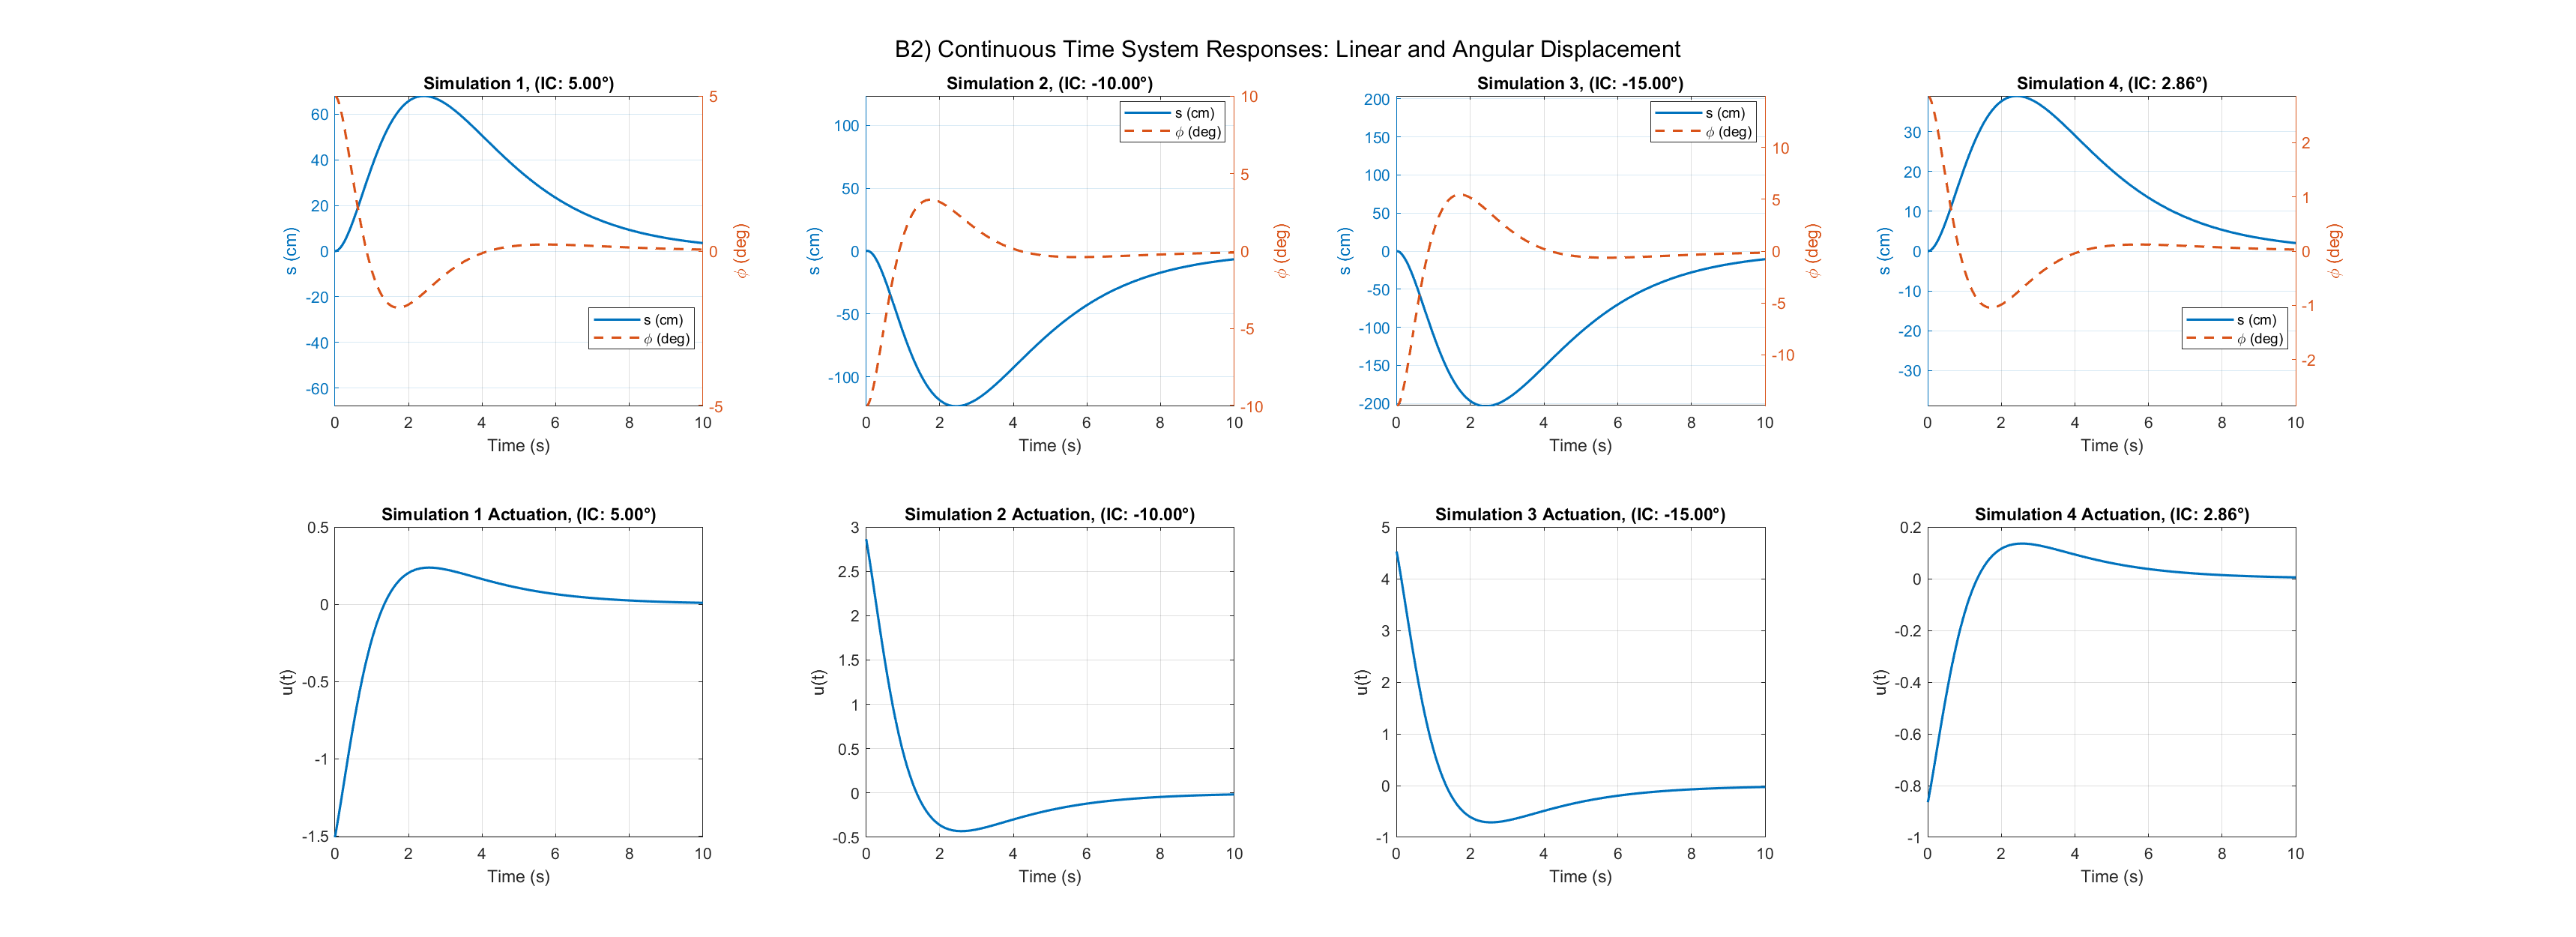
\includegraphics[width=20cm]{figures/b2.png}
    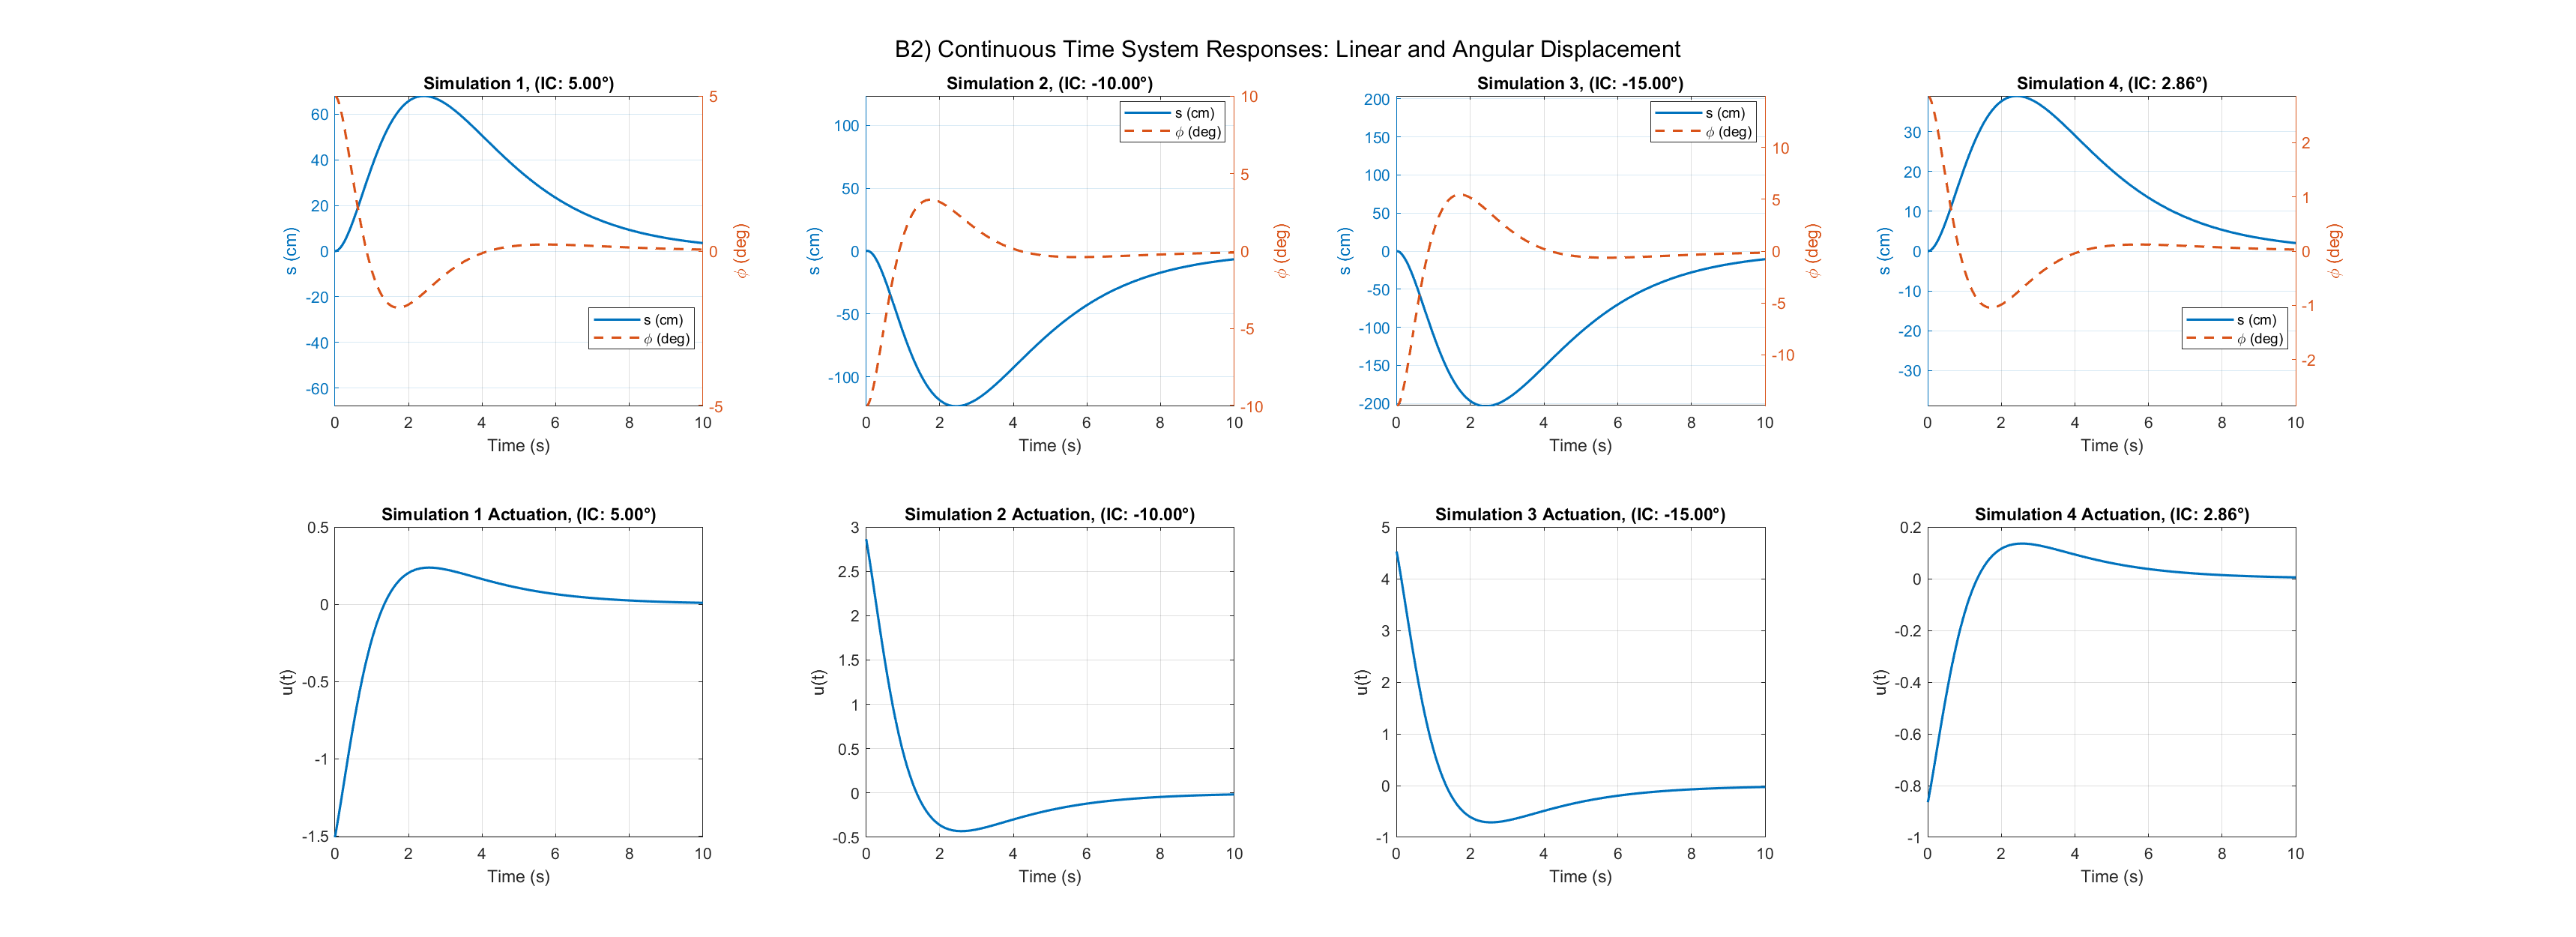
\includegraphics[width=\textwidth]{figures/b2.png}
    \caption{B2) Continuous Time System Responses: Linear and Angular Displacement}
    \label{b2}
\end{figure}

As shown, the controller performance is extremely strong, with the angular rate converging in 5 seconds across all trials with no overshoot or static error. The cart position converges more slowly compared to the pendulum; however, this is not prioritized because the objective is to keep the pendulum upright, not navigate the cart to $s=0$. The maximum experienced velocity of the carts in all simulations is $-1.2m/s$, which was considered within the allowable values, especially when considering that this is when the starting angle was far from the equilibrium position around which the system was linearized. 

\subsection*{B3) Nonlinear Simulation with a Linear Controller}
The same controller was simulated, however this time using the nonlinear differential equation derived in A1. The results are shown in Figure \ref{B3}.

\begin{figure}[H]
    \centering
    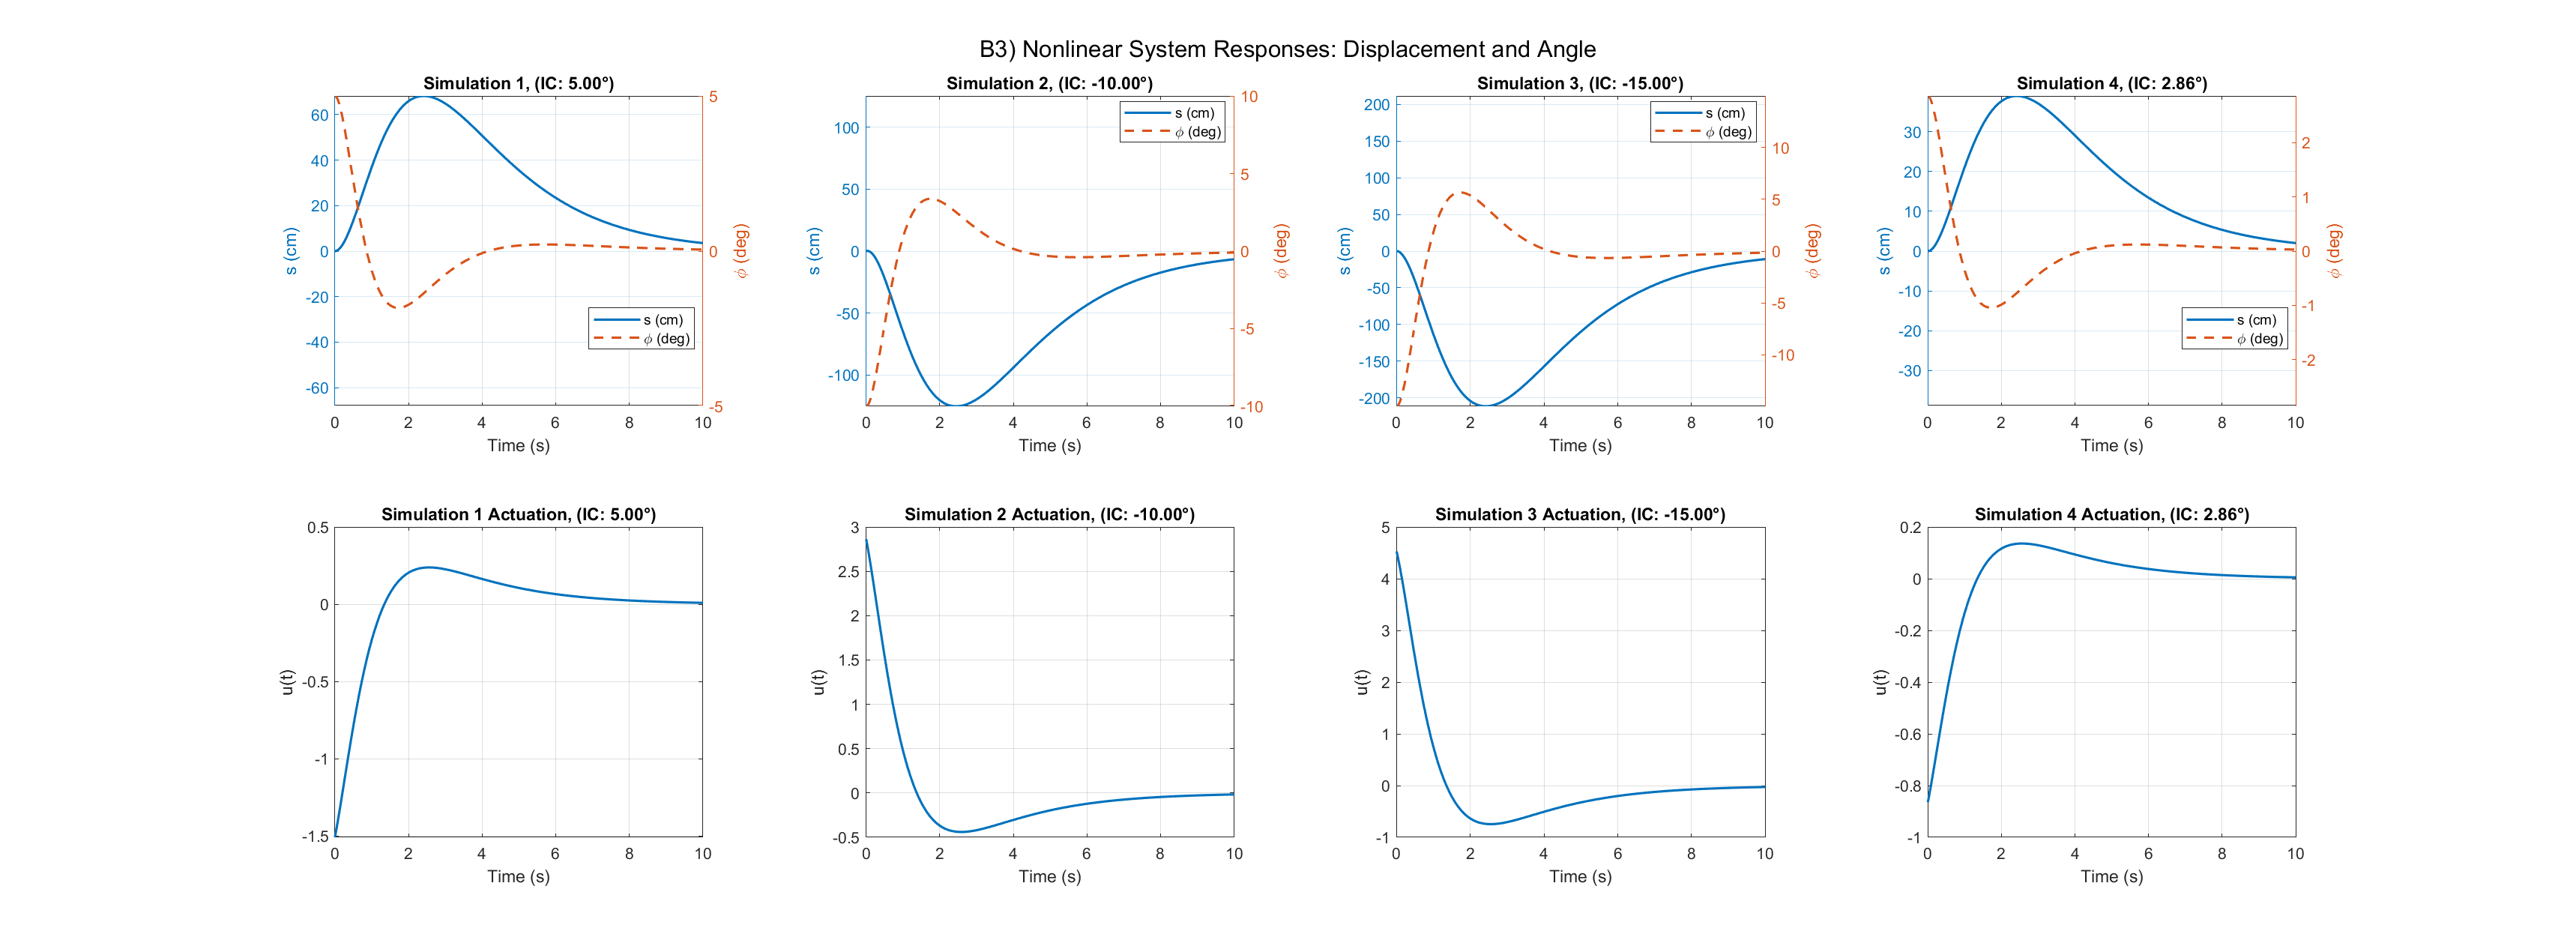
\includegraphics[width=\textwidth]{figures/b3_x.png}
    \caption{B3) Discrete-Time System Responses with an Unstable Sampling Time}
    \label{B3}
\end{figure}

The output of the two state responses are similar; however, in instances where the initial condition deviates far from the point the system was linearized around (simulations 2 and 3), the controller actuates larger movements to try and control the pendulum. Overall, the performance of the controller is still strong across all simulations.

\subsection*{B4) Stable Sampling Time}

To determine the range of allowable sampling time for the linearized system in A3, the system is first digitized to create the closed loop discrete time transfer function. For closed-loop digital stability, all eigenvalues must be in the negative-left side of the complex plane. This maps to the inside of the unit circle in the $z$-plane.
\newline

To derive this value, the known transformations $ A_d=e^{S*Ts}$ is used to create a symbolic representation of the discretized system. The corresponding value of $B_d$ is found identically to as shown in equation \ref{Bd}, however with the sampling time left as a parameter. The determinant of the matrix $A_d+B_dK_d$ (the closed loop feedback state space equation) was found, and its only root is the maximum allowable sampling frequency. This was found to be 1.3707 seconds. Selecting Ts larger than this value lead to the exponential terms not being decaying functions, indicating the instabilities that will begin to arise.
\newline

To show the affect of this instability, the sampling time was set to the maximum allowable sampling frequency, and simulated (Figure \ref{B4}). As expected, when very close to the equilibrium position (Simulations 1 and 4) the controller is somewhat able to balance the pendulum, however there are persistent oscillations indicating the equilibrium is not stable. However once bigger perturbations from the equilibrium state are introduced, the system becomes incredibly unstable, diverging from equilibrium within 2 seconds.

\begin{figure}[H]
    \centering
    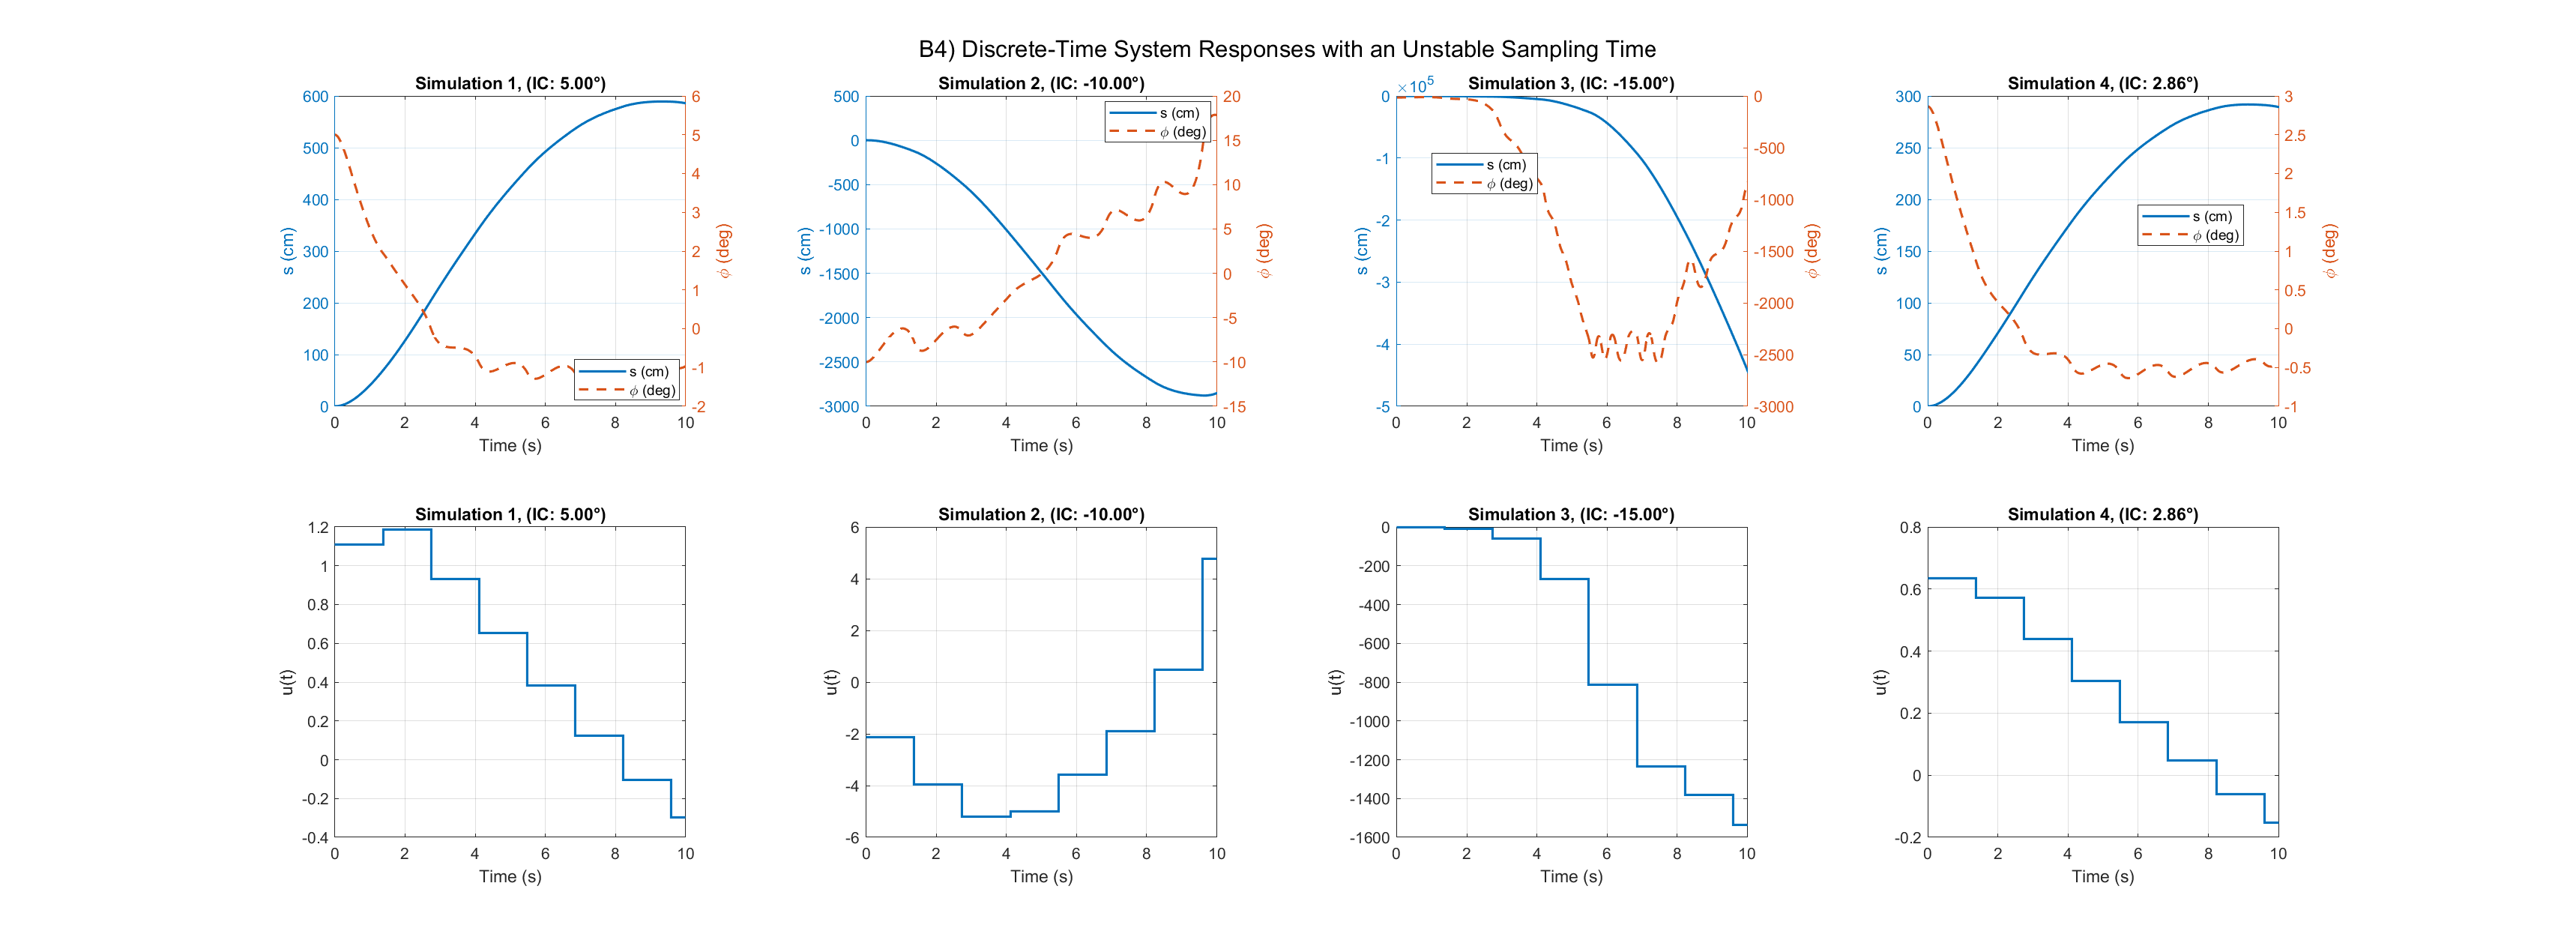
\includegraphics[width=\textwidth]{figures/B4.png}
    \caption{B4) Discrete-Time System Responses with an Unstable Sampling Time ($Ts=1.37$)}
    \label{B4}
\end{figure}



\subsection*{B5) Performance Degradation Across Sampling Times}

The non-linear system was simulated using the same discrete time controller, sampled across a variety of sampling times. The experiment was run across 6 trials, all shown in Figure \ref{B5}, with the sampling time increasing every iteration.

\begin{figure}[H]
    \centering
    \includegraphics[width=\textwidth]{figures/b5.png}
    \caption{B5) Nonlinear System Responses to a Digital Controller with Different Sampling Frequencies}
    \label{B5}
\end{figure}

As expected, systems with sampling times of less than 1 second (80\% of the maximum sampling interval), the controller is able to stabilize the system with relative ease and converges to an equilibrium quickly. Simulation 4 shows a sampling frequency just under the maximum allowable interval. The system can still be stabilized, however the motion is no longer smooth, especially regarding the angular displacement being bery choppy. Simulations 5 and 6 are above the allowable sampling frequency, and show a complete lack of control over the pendulum, which is expected for this system


\subsection*{B6) Discrete Time State Space Representation}
Matrices $A$ and $B$ were calculated in Equations \ref{jacobian} and \ref{jB} respectively. Section B4 noted that the slowest possible sampling time for this system is 1.3707to guarantee asymptotic stability. To introduce a non-unity safety factor, a sampling time of 0.2 was chosen for all future simulations to ensure behavior is as expected from the theoretical derivations of the controller.

To create the discrete-time state-space representation of the cart pendulum system, the following definitions are used to write the system as $\dot x[k+1]=A_dx[k]+B_du[k]$. Equations \ref{ad} and \ref{Bd} show the creation of matrices $A_d$ and $B_d$ respectively.

\begin{equation}\label{ad}
    A_d=e^{\n\left(\begin{array}{cccc} 0 & 1 & 0 & 0\\ 0 & -\frac{F}{M} & 0 & 0\\ 0 & 0 & 0 & 1\\ 0 & \frac{F}{LM} & \frac{g}{L} & 0 \end{array}\right)
\n*Ts}=\begin{bmatrix}
1.0000 & 0.2398 & 0.0000 & 0.0000 \\
0.0000 & 0.7602 & 0.0000 & 0.0000 \\
0.0000 & 0.0440 & 1.4707 & 0.3159 \\
0.0000 & 0.3312 & 3.6807 & 1.4707
\end{bmatrix}

\end{equation}


\begin{equation}\label{Bd}
    B_d=\int_{0}^{T} e^{A(T - \tau)} B \, d\tau=\begin{bmatrix}
1.1353 \\
0.8647 \\
-36.3276 \\
-124.0599
\end{bmatrix}

\end{equation}

It is noted that $C_d=C$ and $D_d=D$ as these matrices do not introduce any new dynamics to the system.



\subsection*{B7) Discrete Time Feedback Controller}
To create a full-state feedback controller for the new discrete-time system, an identical method to that in Section B1, however, the poles are mapped to their discrete-time equivalent. The poles are mapped into the discrete-time variant by first observing that the poles are points on the positive real axis, and thus are in the Laplace ($s$) domain. These can be converted into their respective $z$ representation using $z=e^{sT}$, with sampling time $T$. This maps the poles to the $z$ plane, the new poles being \begin{bmatrix}
0.9048 & 0.8187 & 0.7408 & 0.6703
\end{bmatrix}
. 
\newline

These poles have been mapped from the negative-real axis $\Re^-$, where is the stable Laplacian plane, to now the inside of the unit circle, $D^-$, which is known as the "region of convergence". This is where the poles need to be for the discrete time system to be asymptotically stable. This is expected, as both the sampling time of 0.2s and the poles of the continuous system are stable, and thus it is expected that the poles of the discrete-time system also result in a stable system. Figure \ref{B7} shows the outputted plot for the discrete time linear system.

\begin{figure}[H]
    \centering
    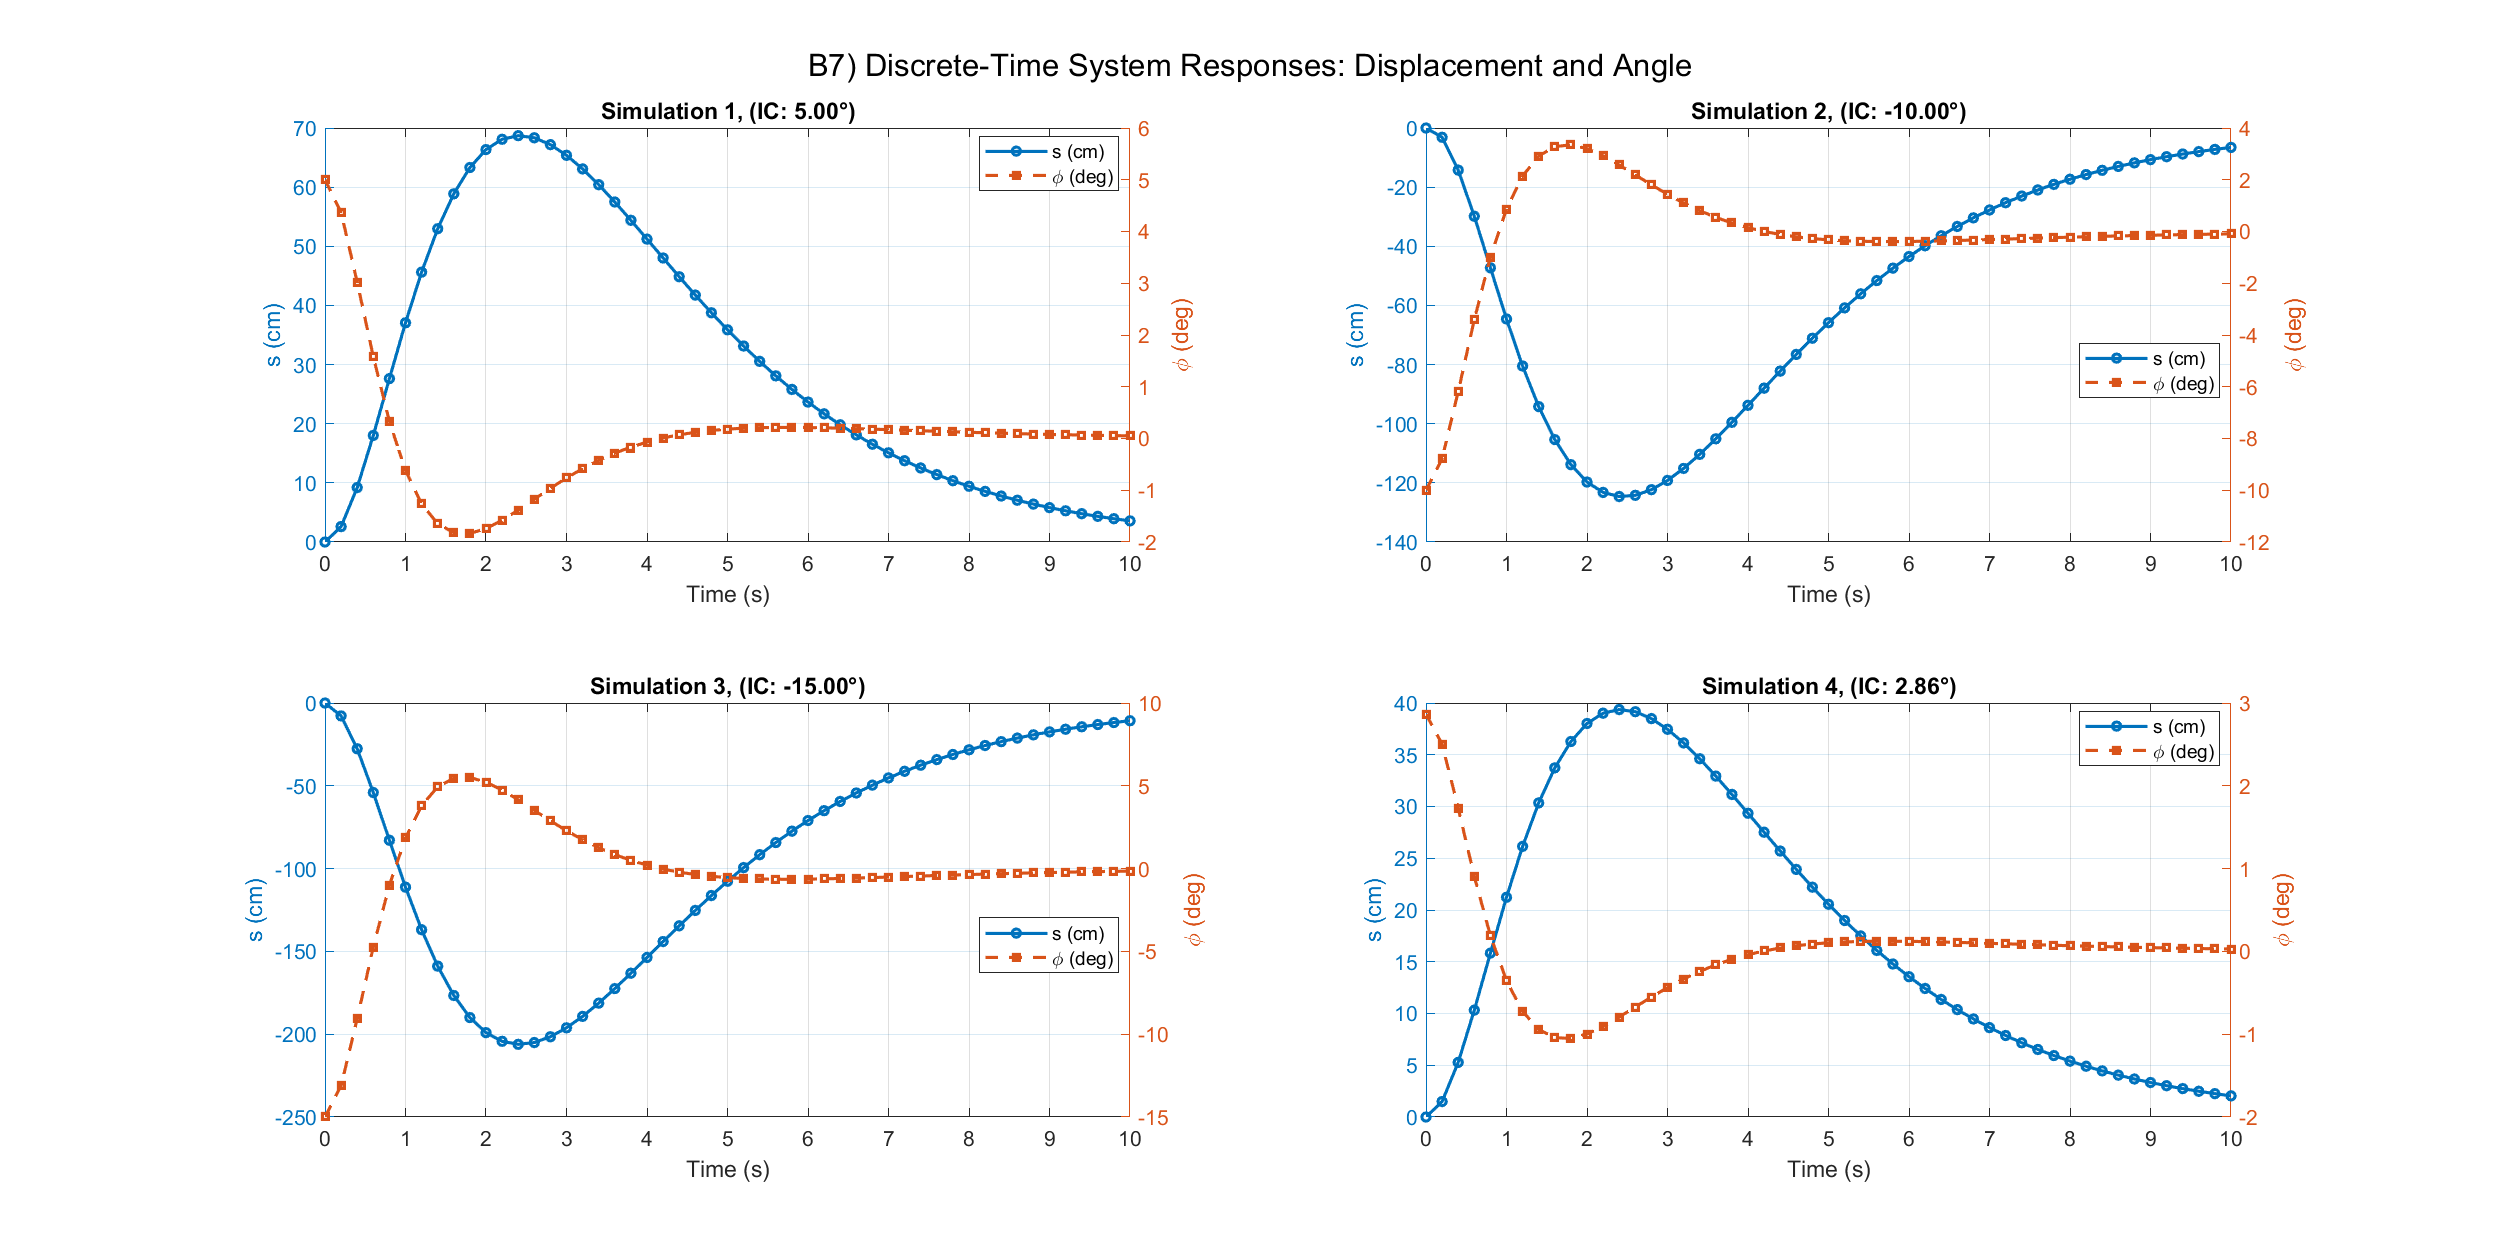
\includegraphics[width=\textwidth]{figures/B7_x.png}
    \caption{B7) Discrete-Time System Responses: Displacement and Angle}
    \label{B7}
\end{figure}

As expected, both systems converge to the equilibrium $\underline{\dot x}=\underline{0}$, with similar performance to before, whereby the angular position (the pendulum being upright) converges much faster than the linear displacement of the cart. This is done by design, as the objective of the experiment is to keep the pendulum upright, rather than move the cart to $s=0$. The performance of this is similar to that observed in Figure \ref{B3}, and this is expected since the same controller is used between both systems, one in discrete time and one in continuous time.

\subsection*{B8) Discrete Time Nonlinear Simulation}
The same digital controller was run, however instead of using the discrete time system, the non-linear system was used, which is the true numerical representation of the system's dynamics. The simulations were run using a non-linear simulator, to capture the true dynamics of the system. Figure \ref{B8} shows the outputted linear and angular displacement, as well as the actuation.

\begin{figure}[H]
    \centering
    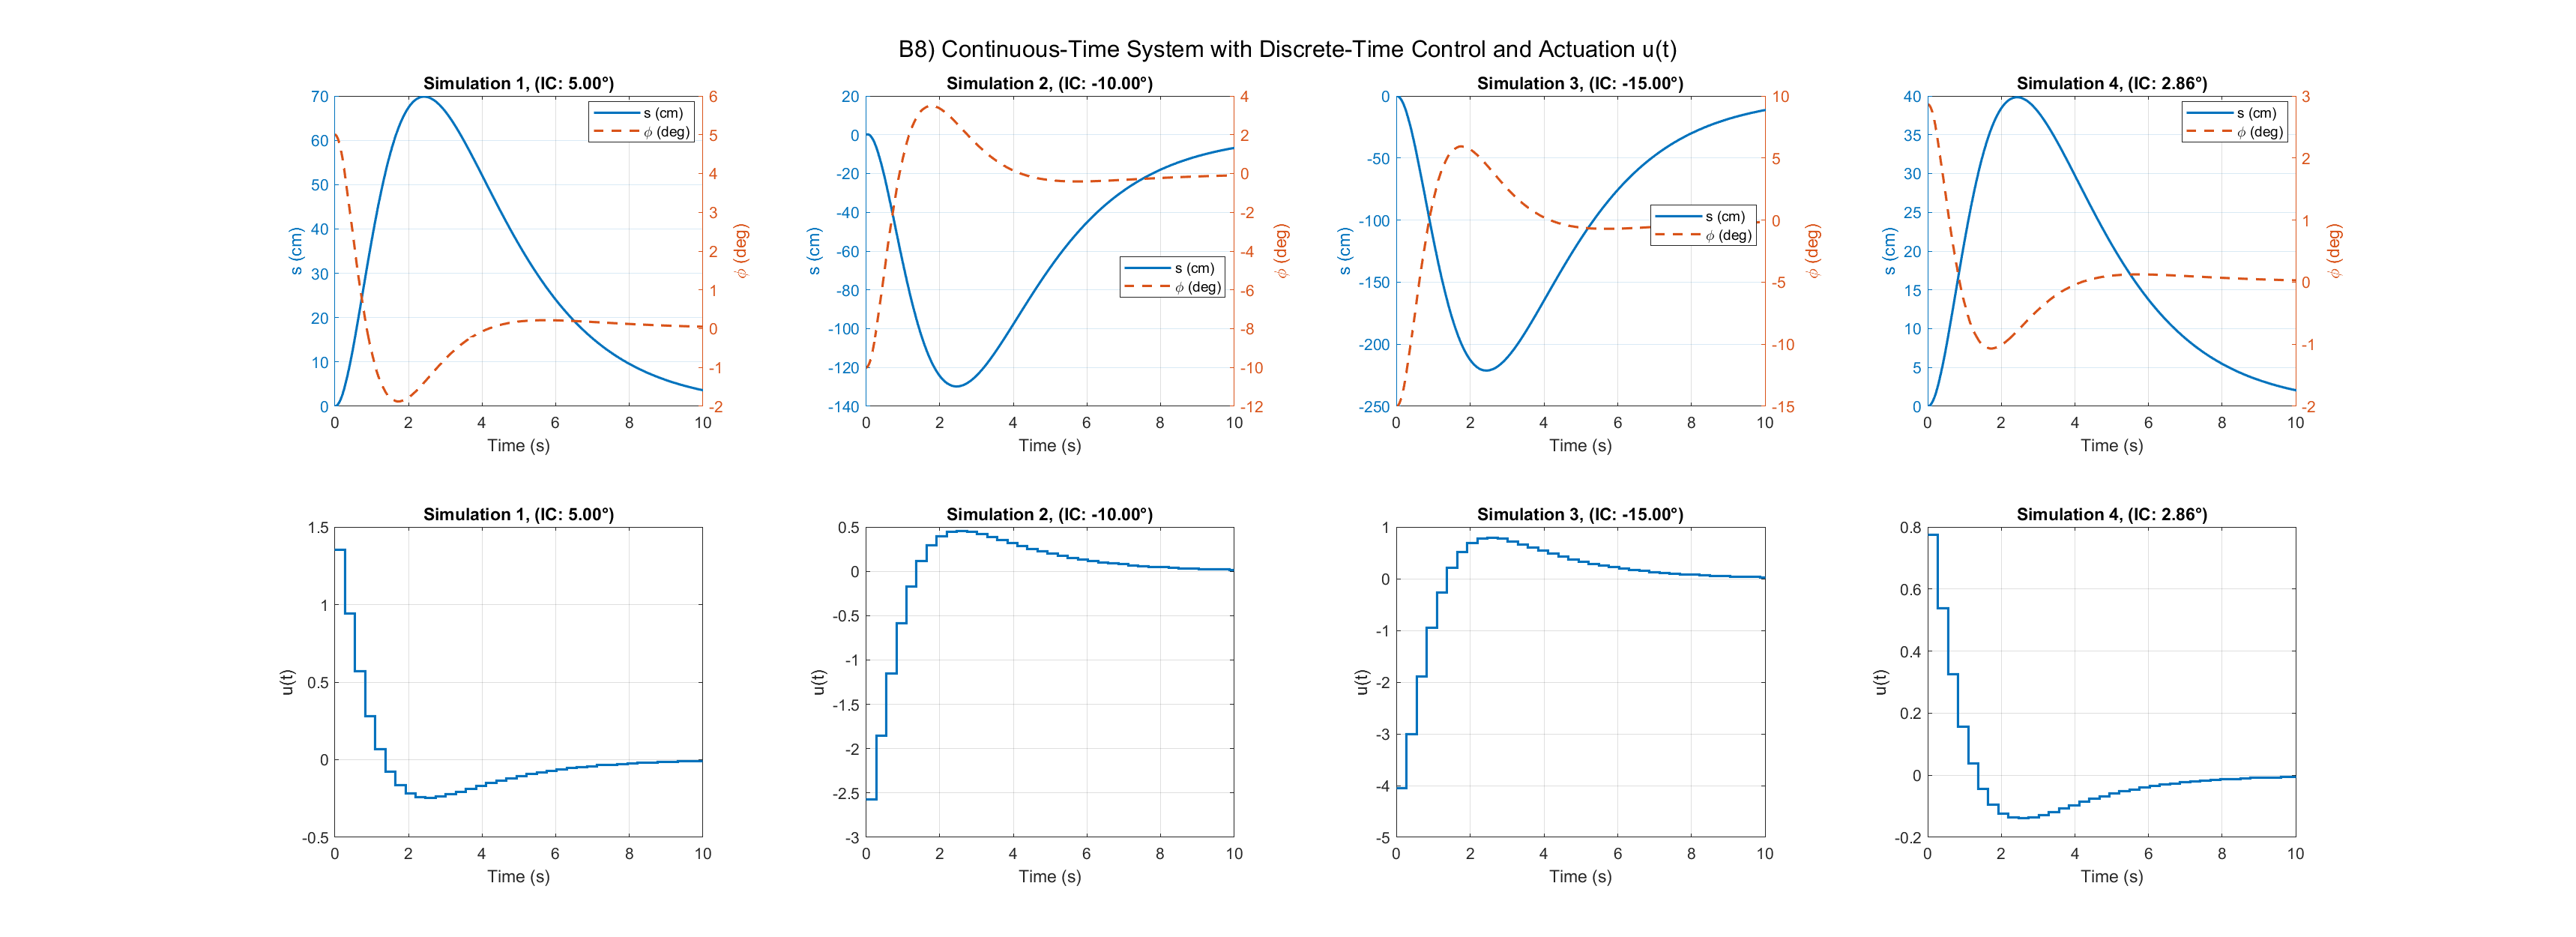
\includegraphics[width=\textwidth]{figures/b8.png}
    \caption{B8) Continuous-Time System with Discrete-Time Control and Actuation}
    \label{B8}
\end{figure}


something here about comparing to b5

\subsection*{B9) Optimal Discrete Time Controller}
An optimal controller is one that minimizes the value of a cost function in relation to a forward trajectory. Optimal controllers are commonly used in model predictive control, whereby the controller needs to find the perfect balance between future states, and input actuation. The cost function must be strictly positive and well defined (with a smooth gradient) to converge on a single, optimal controller. The chosen cost function is shown in Equation \ref{costfn}, and is a quadratic cost. The matrix $Q$ is chosen to be $diag([100, 1, 100, 1])$, such that the position of the cart and the angle of the pendulum are weighted 100 times more than their respective velocities.

\begin{equation}\label{costfn}
    J = \sum_{k=0}^{\infty} \left( x^T(k) Q x(k) + u^T(k) u(k) \right)
\end{equation}

The input is squared to ensure that it is strictly positive and the state is not compared to any reference, as the cost function is minimum when $\underline{x}=\underline{0}$, which is the desired target state. Matlab has built in functionality to solve the algebraic Riccati equation for a standard quadratic function, which Equation \ref{costfn} is, when substituting $R=[1]$. Numerically solving this equation gives the final optimal controller $K^*_d=\begin{bmatrix}
-2.3207 & -3.9491 & -28.9399 & -8.4546
\end{bmatrix}
$.
\newline

The optimal discrete time controller is simulated using the discretized linear system, and the output waveforms are shown in Figure \ref{B9}.

\begin{figure}[H]
    \centering
    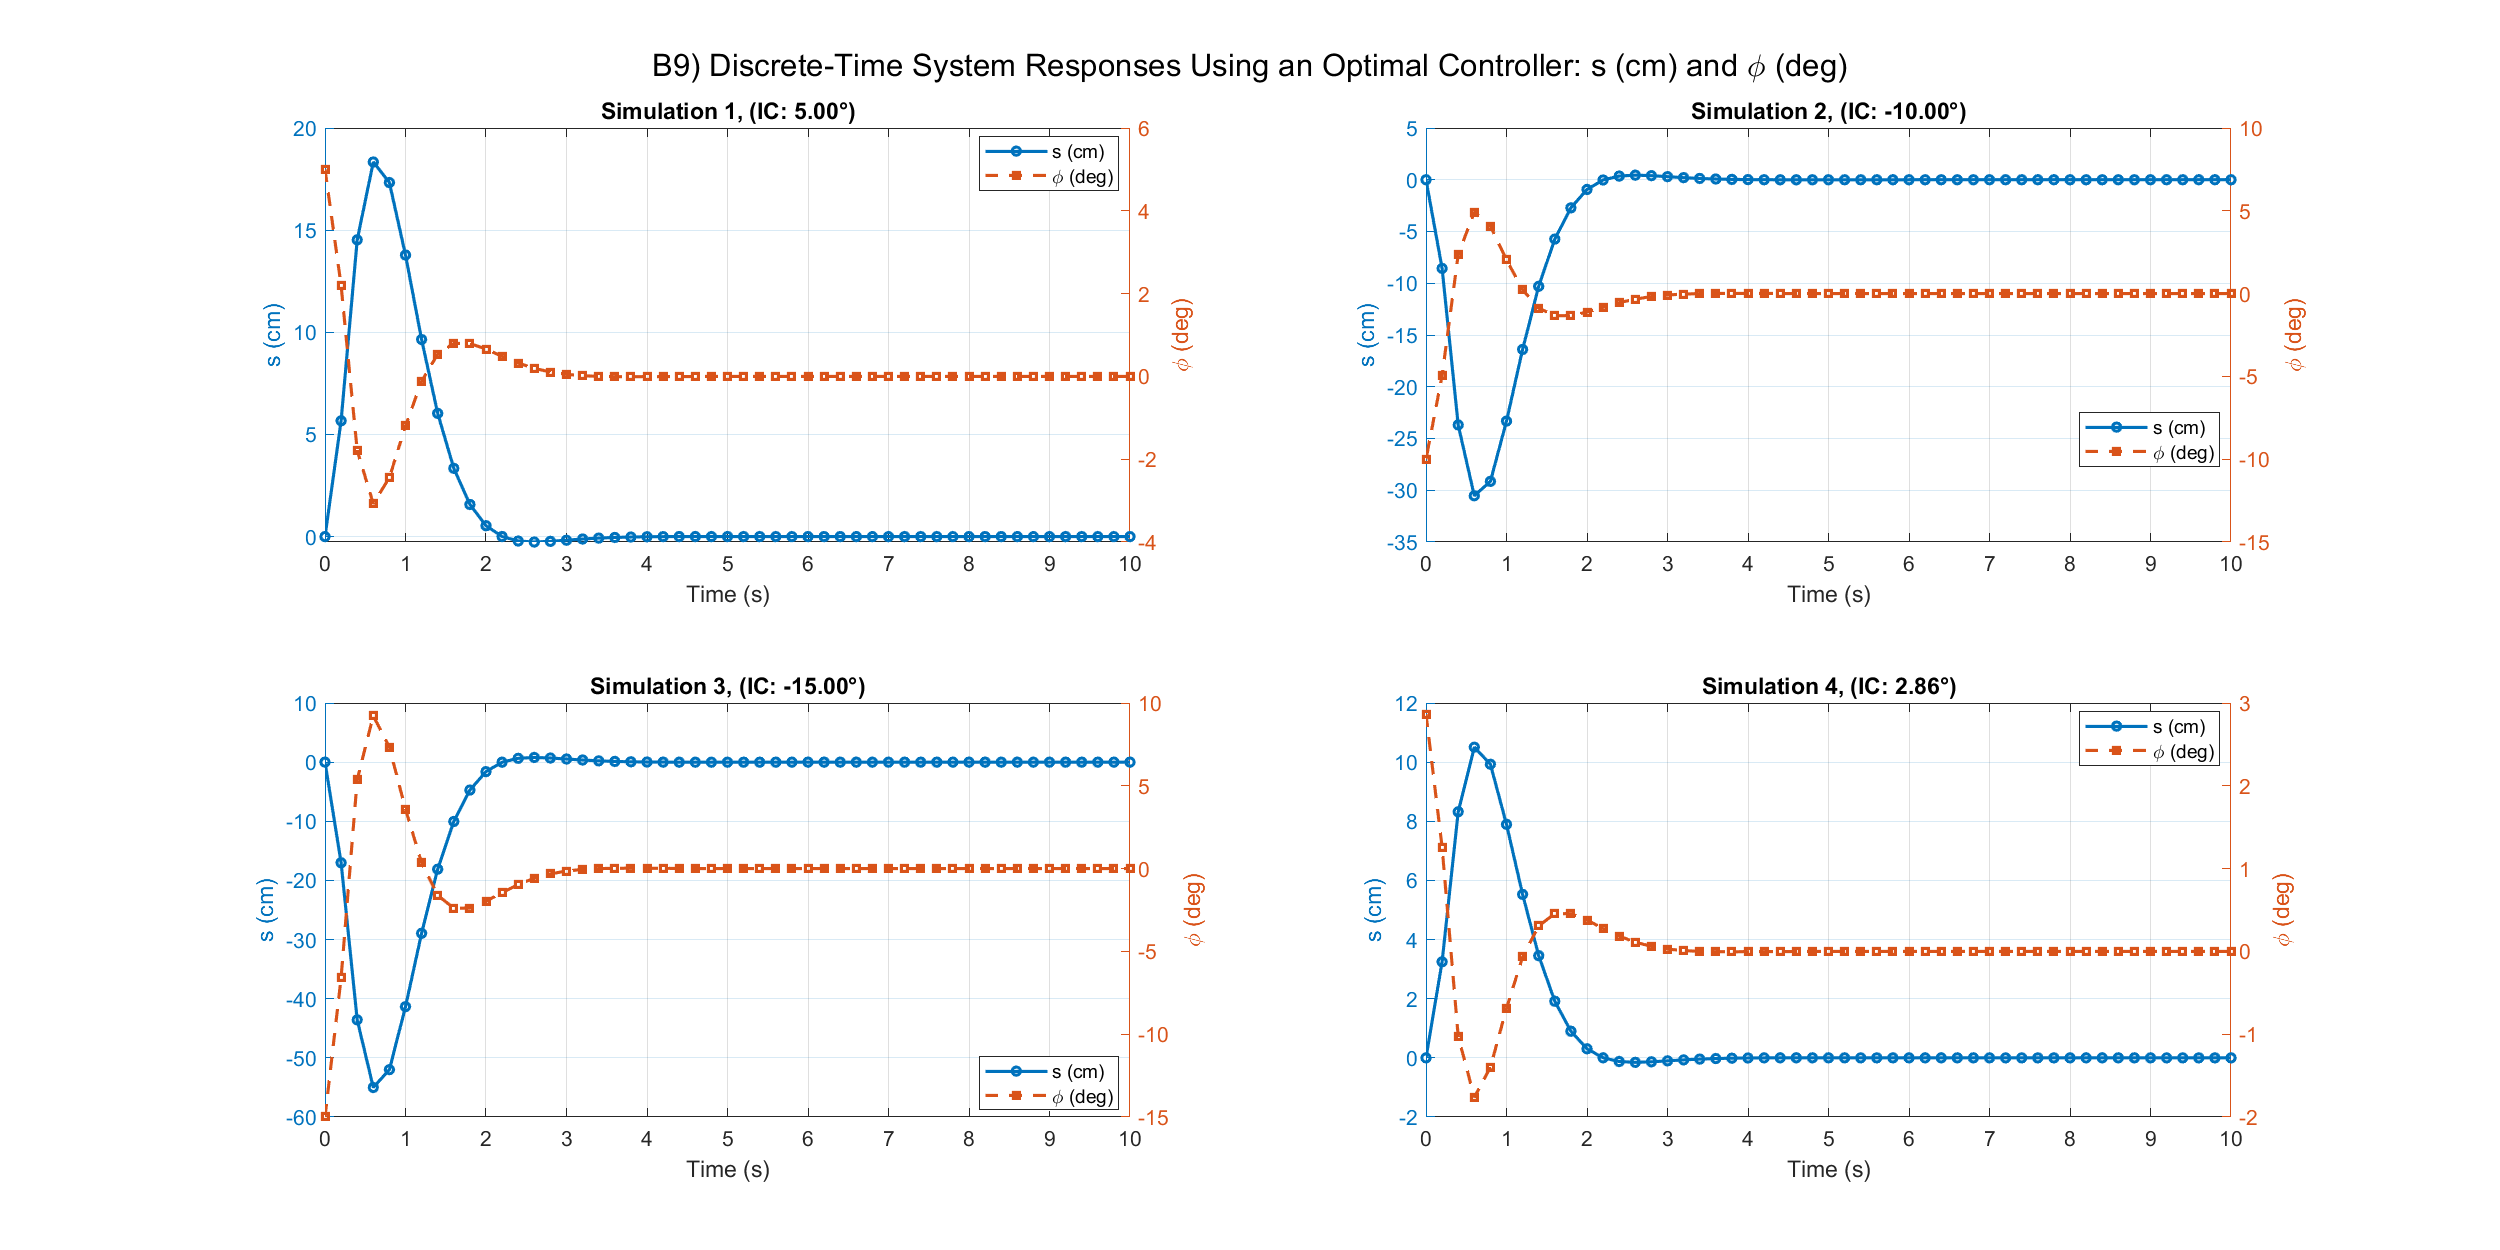
\includegraphics[width=\textwidth]{figures/b9.png}
    \caption{B9) Discrete-Time System Responses Using an Optimal Controller}
    \label{B9}
\end{figure}

Compared to Figures \ref{B3} and \ref{B7}, the performance of this controller is incredibly strong, with convergence of both the angular and linear displacement happening within 2 seconds. Furthermore, the magnitude of the actuation are much smaller than previous values, with the fastest recorded velocity being less than $1 m/s$ (40\% improvement). This is expected, as controller $K^*_d$ is designed to be the best possible controller given the current constraints.

\subsection*{B10) Optimal Discrete Time Controller on Continuous Time Nonlinear Simulation}
The optimal controller was now simulated using the nonlinear model, which most accurately represents the systems dynamics. The expectation is that performance will be similar because of the choice of an appropriate sampling time in conjunction with a safety factor.

\begin{figure}[H]
    \centering
    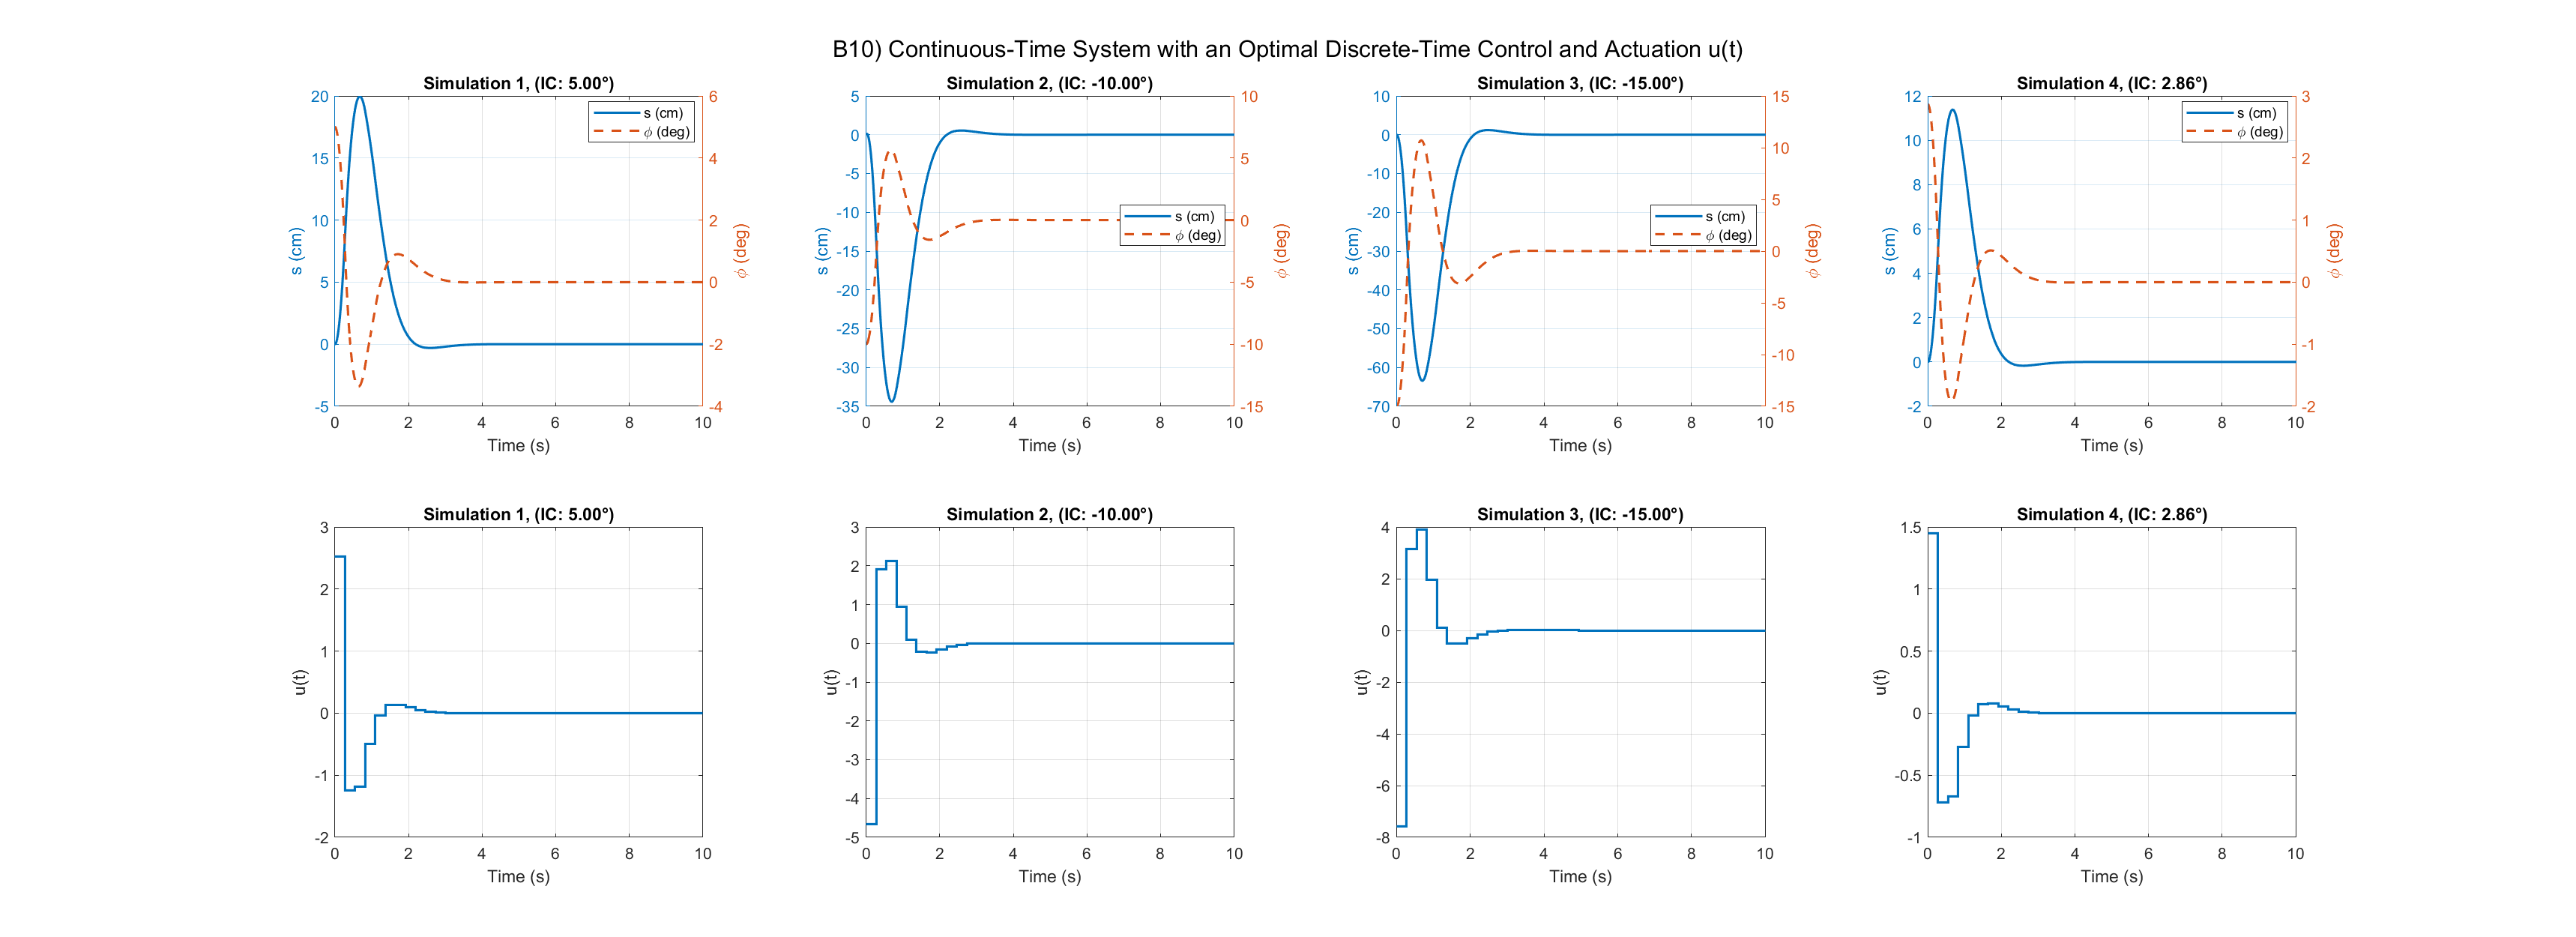
\includegraphics[width=\textwidth]{figures/b10.png}
    \caption{B10) Continuous-Time System with an Optimal Discrete-Time Control and Actuation}
    \label{B10}
\end{figure}

Compared to both B5 and B8, B10 (Figure \ref{B10}) has by far the best performance of any controller designed. The compared metrics are: maximum deviation from equilibrium: settling time, and static error. Controller B10 is approximately 200\% faster at converging to stabilizing the pendulum, with almost 800\% faster convergence to the target cart displacement. All controllers have zero static error, which shows that there were no design errors in controllers B5 and B8, only that their values (poles) were not tuned to the optimal values.
\newline

The conclusion for these three simulations are that the best controllers are designed for the system and an optimization algorithm. Simulation B8 was a discrete controller designed for a discrete system, whereas B5 was a discrete controller designed for a continuous time system simulated on a discrete time system. This explains the marginal improvement from B5 to B8, however designing optimal controllers for an application gives the strongest performance across all performance metrics.

\subsection*{B11) Closing Remarks}
Figures \ref{B4} and \ref{B5} show the importance of the sampling time in controller performance in great detail. The simulations move from being almost non-noticable that the simulation is in discrete time, to the simulation being not working, and it being incredibly obvious that the controller is unable to control the system. 
\newline

Another key observation made that significantly improved the results of this coursework was not only finding that the slowest possible sampling frequency is, but then applying a safety factor on top of that barrier to ensure the controller produces smooth and clear motion.
\newline

The final remark for this coursework assignment is the distinction between a controller designed using pole placement, and one designed using an optimal controller. The performance difference between these two controller is incredibly noticeable, and takes the controller from being incredibly mediocre, to creating the smoothest possible motion and converging on a solution almost $300\%$ faster than any other solution.
\newline

The choice of sampling time in a digital controller significantly impacts controller performance, and should not be an after thaught in controller design.



\newpage
\appendix

\section{GitHub}

All code is available in the below github repository.
\begin{verbatim}
    https://github.com/OmarBenGacem/Digital_Control_Systems_Coursework
\end{verbatim}


\section{Code}
\begin{verbatim}
close all;
clc;
clear;
addpath("analytic_work\");
%% Define symbolic variables
% syms s s_dot phi phi_dot      
% syms u F M m g L      

%% Varaibles
s = sym("s");
t = sym("t");
s_dot = sym("s_dot");
phi = sym("phi");
phi_dot = sym("phi_dot");
F = sym("F");
M = sym("M");
m = sym("m");
g = sym("g");
L = sym("L");
A = sym("A", [4,4]);

%% Functions
x = symfun(sym("x", [4,1]), t);
x_dot = diff(x(t), t);
u = symfun(sym("u"), t);


x = [s; s_dot; phi; phi_dot];


x_eq = [0; 0; 0; 0];
u_eq = 0; 


s_dot_eq   = s_dot;
s_ddot_eq  = - (F/M)*s_dot + u/M;
phi_dot_eq = phi_dot;
phi_ddot_eq= ( (g/L) * sin(phi) ) + ( (F/(M*L)) * s_dot * cos(phi) ) - ( u/(L*M) * cos(phi) ) ;

x_dot = [s_dot_eq; s_ddot_eq; phi_dot_eq; phi_ddot_eq];

A_sym = jacobian(x_dot, x);

B_sym = jacobian(x_dot, u);
A = subs(A_sym, [s, s_dot, phi, phi_dot, u], [x_eq.' u_eq]);
B = subs(B_sym, [s, s_dot, phi, phi_dot, u], [x_eq.' u_eq]);


C = [1 0 0 0;
     0 0 1 0];
D = zeros(2, 1);

save("a3", "A", "B", "C", "D");

R = sym("R");
O = sym("O");
Reachability_Matrix = [B , A*B , A^2*B , A^3*B];
Observability_Matrix = [C ; C*A];
Linear_Dynamics = [A , B ; C , D];


toOverleaf(eye(2), "test", true)
toOverleaf(A, "A", true);
toOverleaf(B, "B", true);
% toOverleaf(Reachability_Matrix, "reachability", true);
% toOverleaf(Observability_Matrix, "observability", true);
toOverleaf(Reachability_Matrix, "reachability", true);
toOverleaf(Observability_Matrix, "observability", true);
toOverleaf(Linear_Dynamics, "linear_dynamics", true);

if false
    toOverleaf(det(Reachability_Matrix),"reachability_det", false)
    % toOverleaf(det(Observability_Matrix),"observability_det") 
end

% toOverleaf(C, "C");
% toOverleaf(D, "D");




%% Constants
M_val = 1;
F_val = 1;
L_val = 0.842;
g_val = 9.8093;


%% Constraints
phi_min_max = pi / 4;
max_lin_v = 5;


plot_B2  = false;
plot_B3  = true;
plot_B4  = true;
plot_B5  = true;
plot_B7  = false;
plot_B8  = false;
plot_B9  = false;
plot_B10 = false;

%                      s     sdot   phi     dphi
initial_conditions = [ 0,   0,     0.0872665,      0;
                       0,     0.1,   -0.174533, 0;   
                       0,     0,     -0.261799,   0;  
                       0,     0,     0.05,   0];  
tspan = [0 10];








%% B1 B2
%  Design a state feedback controller u(t) = Kx(t) which stabilizes the linearized system (2) in x(t) = 0. Comment your design



A_val_sym = subs(A, [F, g, M, L], [F_val, g_val, M_val, L_val]);
B_val_sym = subs(B, [M, L], [M_val, L_val]);

A_val = double(A_val_sym);
B_val = double(B_val_sym);

% poles = [-1, -190, -54, -20]
% poles = [-1, -2, -4, -8];
poles=[-0.5,-1,-1.5,-2];
% toOverleaf(P==poles, "poles");
K = place(A_val, B_val, poles);

A_cl = A_val - B_val*K;


toOverleaf(poles, "poles", true)
toOverleaf(K, "K", true)

if plot_B2

    figure('Position', [100, 100, 2200, 800]);
    nSim = size(initial_conditions, 1);
    
    ax1_all = [];  % Store subplot handles for linking
    ax2_all = [];
    
    for i = 1:nSim
        x0 = initial_conditions(i, :).';
        [t, x] = ode45(@(t, x) A_cl*x, tspan, x0);
    
        % Convert initial condition from radians to degrees
        IC_deg = initial_conditions(i,3) * (180/pi);

        % First subplot: State evolution
        ax1 = subplot(2, nSim, i);
        yyaxis left
        plot(t, x(:,1)*100, '-', 'LineWidth', 1.5)
        ylabel('s (cm)')
    
        % Find symmetric limits for 's (cm)'
        y_left_min = min(x(:,1)*100);
        y_left_max = max(x(:,1)*100);
        y_left_lim = max(abs([y_left_min, y_left_max]));  % Symmetric limit
        ylim([-y_left_lim, y_left_lim]);  % Ensure zero alignment
    
        yyaxis right
        plot(t, x(:,3)*180/pi, '--', 'LineWidth', 1.5)
        ylabel('\phi (deg)')
    
        % Find symmetric limits for 'φ (deg)'
        y_right_min = min(x(:,3)*180/pi);
        y_right_max = max(x(:,3)*180/pi);
        y_right_lim = max(abs([y_right_min, y_right_max]));  % Symmetric limit
        ylim([-y_right_lim, y_right_lim]);  % Ensure zero alignment
    
        title(sprintf("Simulation %d, (IC: %.2f°)", i, IC_deg))  % Updated title with degree symbol
        xlabel('Time (s)')
        grid on;
        legend('s (cm)', '\phi (deg)', 'Location', 'Best')
        xlim([0 t(end)]); 
        ax1_all = [ax1_all, ax1];  % Store handle
    
        % Second subplot: Actuation input
        ax2 = subplot(2, nSim, i + nSim);
        u = K * x';  % Ensure matrix multiplication is correct
        plot(t, u, 'LineWidth', 1.5)
        title(sprintf("Simulation %d Actuation, (IC: %.2f°)", i, IC_deg))  % Updated title with degree symbol
        xlabel('Time (s)')
        ylabel('u(t)')
        grid on;
        xlim([0 t(end)]);
        ax2_all = [ax2_all, ax2];  % Store handle
    end
    
    % Link x-axes for better visualization
    linkaxes([ax1_all, ax2_all], 'x');


    sgtitle('B2) Continuous Time System Responses: Linear and Angular Displacement')
    saveas(gcf, '../figures/b2.png');
end


%% B3

if plot_B3


    figure('Position', [100, 100, 2200, 800]);
    nSim = size(initial_conditions, 1);
    
    ax1_all = [];  % Store subplot handles for linking
    ax2_all = [];
    
    for i = 1:nSim
        x0 = initial_conditions(i, :).';
        [t, x] = ode45(@(t, x) state_update(x, -K*x), tspan, x0);
    
        % Convert initial condition from radians to degrees
        IC_deg = initial_conditions(i,3) * (180/pi);
    
        % First subplot: State evolution
        ax1 = subplot(2, nSim, i);
        yyaxis left
        plot(t, x(:,1)*100, '-', 'LineWidth', 1.5)
        ylabel('s (cm)')
    
        % Find symmetric limits for 's (cm)'
        y_left_min = min(x(:,1)*100);
        y_left_max = max(x(:,1)*100);
        y_left_lim = max(abs([y_left_min, y_left_max]));  % Symmetric limit
        ylim([-y_left_lim, y_left_lim]);  % Ensure zero alignment
    
        yyaxis right
        plot(t, x(:,3)*180/pi, '--', 'LineWidth', 1.5)
        ylabel('\phi (deg)')
    
        % Find symmetric limits for 'φ (deg)'
        y_right_min = min(x(:,3)*180/pi);
        y_right_max = max(x(:,3)*180/pi);
        y_right_lim = max(abs([y_right_min, y_right_max]));  % Symmetric limit
        ylim([-y_right_lim, y_right_lim]);  % Ensure zero alignment
    
        title(sprintf("Simulation %d, (IC: %.2f°)", i, IC_deg))  % Updated title with degree symbol
        xlabel('Time (s)')
        grid on;
        legend('s (cm)', '\phi (deg)', 'Location', 'Best')
        xlim([0 t(end)]); 
        ax1_all = [ax1_all, ax1];  % Store handle
    
        % Second subplot: Actuation input
        ax2 = subplot(2, nSim, i + nSim);
        u = K * x';  % Ensure matrix multiplication is correct
        plot(t, u, 'LineWidth', 1.5)
        title(sprintf("Simulation %d Actuation, (IC: %.2f°)", i, IC_deg))  % Updated title with degree symbol
        xlabel('Time (s)')
        ylabel('u(t)')
        grid on;
        xlim([0 t(end)]);
        ax2_all = [ax2_all, ax2];  % Store handle
    end
    
    % Link x-axes for better visualization
    linkaxes([ax1_all, ax2_all], 'x');


    sgtitle('B3) Nonlinear System Responses: Displacement and Angle')
    saveas(gcf, '../figures/b3_x.png');



    figure('Position', [100, 100, 2200, 800]);
    nSim = size(initial_conditions, 1);
    
    ax1_all = [];  % Store subplot handles for linking
    ax2_all = [];
    
    for i = 1:nSim
        x0 = initial_conditions(i, :).';
        [t, x] = ode45(@(t, x) state_update(x, -K*x), tspan, x0);
    
        % Convert initial condition from radians to degrees
        IC_deg = initial_conditions(i,3) * (180/pi);
    
        % First subplot: State evolution
        ax1 = subplot(2, nSim, i);
        yyaxis left
        plot(t, x(:,2)*100, '-', 'LineWidth', 1.5)
        ylabel('s (cm)')
    
        % Find symmetric limits for 's (cm)'
        y_left_min = min(x(:,2)*100);
        y_left_max = max(x(:,2)*100);
        y_left_lim = max(abs([y_left_min, y_left_max]));  % Symmetric limit
        ylim([-y_left_lim, y_left_lim]);  % Ensure zero alignment
    
        yyaxis right
        plot(t, x(:,4)*180/pi, '--', 'LineWidth', 1.5)
        ylabel('\phi (deg)')
    
        % Find symmetric limits for 'φ (deg)'
        y_right_min = min(x(:,4)*180/pi);
        y_right_max = max(x(:,4)*180/pi);
        y_right_lim = max(abs([y_right_min, y_right_max]));  % Symmetric limit
        ylim([-y_right_lim, y_right_lim]);  % Ensure zero alignment
    
        title(sprintf("Simulation %d, (IC: %.2f°)", i, IC_deg))  % Updated title with degree symbol
        xlabel('Time (s)')
        grid on;
        legend('s (cm)', '\phi (deg)', 'Location', 'Best')
        xlim([0 t(end)]); 
        ax1_all = [ax1_all, ax1];  % Store handle
    
        % Second subplot: Actuation input
        ax2 = subplot(2, nSim, i + nSim);
        u = K * x';  % Ensure matrix multiplication is correct
        plot(t, u, 'LineWidth', 1.5)
        title(sprintf("Simulation %d Actuation, (IC: %.2f°)", i, IC_deg))  % Updated title with degree symbol
        xlabel('Time (s)')
        ylabel('u(t)')
        grid on;
        xlim([0 t(end)]);
        ax2_all = [ax2_all, ax2];  % Store handle
    end
    
    % Link x-axes for better visualization
    linkaxes([ax1_all, ax2_all], 'x');

    sgtitle('B3) Nonlinear System Responses: Angular and Linear Velocities')
    saveas(gcf, '../figures/b3_v.png');

end




%% GO TO BOTTOM FOR PLOTTING B4 AND B5


%% B4
%  Suppose that the control law is implemented with a discrete-time controller connected to the linearized
%  system (2) via an impulsive sampler (sampling the continuous-time state x(t) on one side) and a hold
%  (generating the continuous-time input u(t) on the other side). Find a value of the sampling time T
%  for which the closed-loop system is asymptotically stable. Find a value of T for which the closed-loop
%  system is unstable. Plot the corresponding y(t) and comment on the plots.


    T = sym("T");
    Ad = expm(A * T);
    integrand = expm(A * (T - tau)) * B;
    Bd = int(integrand, tau, 0, T);
    Kd = exp(K * T);
    
    feedback = Ad + Bd * Kd;
    deter = det(feedback(1));
    deter_val = subs(deter, [F, g, M, L, K], [F_val, g_val, M_val, L_val, place(A_val, B_val, poles)]);

    Ts_max = double(solve(0 == deter_val))




safety_factor = 5;
Ts = Ts_max / safety_factor


%% B5
%  Similarly to point B4, apply the discrete-time control law to the nonlinear system (1). This time,
%  focus and discuss about the possible degradation in performance for different values of T. Display
%  plots of y(t) and comment on the plots.

if plot_B5

    Kd = sym("Kd", [1,4]);
    
    Ts_vals = linspace(0.1, 2, 6);
    
    initial_condition_num = 2;
    state0 = initial_conditions(initial_condition_num, :).'; 
    IC_deg = initial_conditions(initial_condition_num,3) * (180/pi);
    
    figure('Position', [100, 100, 2200, 800]);
    
    for j = 1:length(Ts_vals)
        Ts = Ts_vals(j);  
   
        Ad = expm(A_val * Ts);
        Bd = double( int(expm(A_val * (Ts - tau)) * B_val, tau, 0, Ts) ); 
    

        poles_discrete = exp(poles * Ts);
        Kd = place(Ad, Bd, poles_discrete);
    
        A_d_cl = Ad - Bd * Kd;

        toOverleaf(poles_discrete, sprintf("poles_d_T%.2f", Ts), true);
        toOverleaf(Kd, sprintf("Kd_T%.2f", Ts), true);
    
        t_sim = tspan(1):Ts:tspan(end);
        x_hist = zeros(4, length(t_sim)); 
        state = state0;
    
        for idx = 1:length(t_sim)
            x_hist(:, idx) = state;
            state = A_d_cl * state;
        end
    
        % Plot
        subplot(2, 3, j)
        yyaxis left
        plot(t_sim, x_hist(1, :)*100, 'o-', 'LineWidth', 1.5, 'MarkerSize', 4)
        ylabel('s (cm)')
    
        yyaxis right
        plot(t_sim, x_hist(3, :)*180/pi, 's--', 'LineWidth', 1.5, 'MarkerSize', 4)
        ylabel('\phi (deg)')
    
        title(sprintf("Simulation With Ts = %.2f s", Ts, IC_deg))
        xlabel('Time (s)')
        grid on
        legend('s (cm)', '\phi (deg)', 'Location', 'Best')
    end
    
    sgtitle('B5) Discrete-Time System Responses for Varying Sampling Time')
    saveas(gcf, '../figures/B5.png');



end


%% B6
%  A bunch of equations


Ad = expm((A_val * Ts));
% syms tau
% Bd = int(expm(A_val * (Ts - tau)) * B_val, tau, [0, Ts]);
Bd = integral( @(tau) expm(A_val * (Ts - tau)  ) * B_val, 0, Ts, 'ArrayValued', true );
Cd = C;
Dd = D;

toOverleaf(Ad, "Ad", true);
toOverleaf(Bd, "Bd", true);
toOverleaf(Cd, "Cd", true)
toOverleaf(Dd, "Dd", true);


%% B7
%  Design a discrete-time state feedback control law u(k) = Kdx(k) such that the closed-loop associated
%  to the discretized linearized system computed in point B6 is asymptotically stable (Hint: place the
%  poles of Ad + KdBd mapping the eigenvalues you chose in point B1 to the z-plane). Display plots
%  of y(t) and comment on the plots.


Kd = sym("Kd", [1,4]);
poles_discrete = exp(poles * Ts);
Kd = place(Ad, Bd, poles_discrete);

A_d_cl = Ad - Bd * Kd; 


toOverleaf(poles_discrete, "poles_d", true);
toOverleaf(Kd, "Kd", true);



if plot_B7
    
    figure('Position', [100, 100, 1600, 800]);
    
    for i = 1:size(initial_conditions,1)
       IC_deg = initial_conditions(i,3) * (180/pi);
        state = initial_conditions(i, :).';  % Column vector

        t_sim = tspan(1):Ts:tspan(end);
        x_hist = zeros(4, length(t_sim)); 

        % Simulate the discrete-time system
        for idx = 1:length(t_sim)
            x_hist(:, idx) = state;
            state = A_d_cl*(state);
        end

        subplot(2,2,i)
        yyaxis left
        plot(t_sim, x_hist(1, :)*100, 'o-', 'LineWidth', 1.5, 'MarkerSize', 4) % Discrete points
        ylabel('s (cm)')

        yyaxis right
        plot(t_sim, x_hist(3, :)*180/pi, 's--', 'LineWidth', 1.5, 'MarkerSize', 4) % Discrete points
        ylabel('\phi (deg)')
        
        title(sprintf("Simulation %d, (IC: %.2f°)", i, IC_deg))
        xlabel('Time (s)')
        grid on;
        legend('s (cm)', '\phi (deg)', 'Location', 'Best')
    end
    
    sgtitle('B7) Discrete-Time System Responses: Displacement and Angle')
    saveas(gcf, '../figures/B7_x.png');


    figure('Position', [100, 100, 1600, 800]);
    for i = 1:size(initial_conditions,1)
        IC_deg = initial_conditions(i,3) * (180/pi);

        state = initial_conditions(i, :).';


        t_sim = tspan(1):Ts:tspan(end);
        x_hist = zeros(4, length(t_sim));

        for idx = 1:length(t_sim)
            x_hist(:, idx) = state; 
            state = A_d_cl*(state); 
        end

        subplot(2,2,i)
        yyaxis left
        plot(t_sim, x_hist(2, :)*100, 'o-', 'LineWidth', 1.5, 'MarkerSize', 4)
        ylabel('Linear Velocity (cm/s)')

        yyaxis right
        plot(t_sim, x_hist(4, :)*180/pi, 's--', 'LineWidth', 1.5, 'MarkerSize', 4)
        ylabel('Angular Velocity (deg/s)')
        
        title(sprintf("Simulation %d, (IC: %.2f°)", i, IC_deg))
        xlabel('Time (s)')
        grid on;
        legend('cm/s', 'rad/s', 'Location', 'Best')
    end
    
    sgtitle('B7) Discrete-Time System Responses: Linear and Angular Velocities')
    saveas(gcf, '../figures/B7_v.png');



end




%% B8
%  Apply the discrete-time state feedback control law u(k) = Kdx(k) to the continuous-time nonlinear
%  system (1) (obviously sampling the state and holding the input). Display plots of y(t), comment on
%  the plots and compare with the results of point B5.

if plot_B8
    figure('Position', [100, 100, 2200, 800]);
    nSim = size(initial_conditions, 1);
    
    for i = 1:nSim
        IC_deg = initial_conditions(i,3) * (180/pi);


        x0 = initial_conditions(i, :).';
        t_total = [];
        x_total = [];
        t_u = []; 
        u_total = []; 
        
        t_offset = 0;
        T_final = tspan(end); 
        N_intervals = ceil(T_final / Ts);
        
        for k = 1:N_intervals

            u = -Kd * x0;
            [t_interval, x_interval] = ode45(@(t, x) state_update(x, u), [0 Ts], x0);
           
            t_interval = t_interval + t_offset;

            t_total = [t_total; t_interval];
            x_total = [x_total; x_interval];

            t_u = [t_u; t_offset; t_offset + Ts];
            u_total = [u_total; u; u];

            x0 = x_interval(end, :)';
        
            t_offset = t_offset + Ts;
        end
      
        ax1 = subplot(2, nSim, i);
        yyaxis left
        plot(t_total, x_total(:,1)*100, '-', 'LineWidth', 1.5)
        ylabel('s (cm)')
        yyaxis right
        plot(t_total, x_total(:,3)*180/pi, '--', 'LineWidth', 1.5)
        ylabel('\phi (deg)')
        title(sprintf("Simulation %d, (IC: %.2f°)", i, IC_deg))
        xlabel('Time (s)')
        grid on;
        legend('s (cm)', '\phi (deg)', 'Location', 'Best')
        xlim([0 T_final]); 
        ax2 = subplot(2, nSim, i+nSim);
        stairs(t_u, u_total, 'LineWidth', 1.5)
        title(sprintf("Simulation %d, (IC: %.2f°)", i, IC_deg))
        xlabel('Time (s)')
        ylabel('u(t)')
        grid on;
        xlim([0 T_final]);

        linkaxes([ax1, ax2], 'x');
    end
    
    sgtitle('B8) Continuous-Time System with Discrete-Time Control and Actuation u(t)')
    saveas(gcf, '../figures/b8.png');
end







%% B8
%  Apply the discrete-time state feedback control law u(k) = Kdx(k) to the continuous-time nonlinear
%  system (1) (obviously sampling the state and holding the input). Display plots of y(t), comment on
%  the plots and compare with the results of point B5.





%% B9
%  A bunch of equations


if plot_B9
    
    figure('Position', [100, 100, 1600, 800]);
    for i = 1:size(initial_conditions,1)
        IC_deg = initial_conditions(i,3) * (180/pi);
        

        state = initial_conditions(i, :).';
        init = initial_conditions(i, :).';
        save("digital_values.mat","Ad","Bd", "tspan", "Ts", "init");
        Kd_star = fminsearch(@optimization_problem, Kd);
        toOverleaf(Kd_star, "kdstar", true);
        delete("digital_values.mat")
        A_d_cl_star = ((Ad - Bd * Kd_star)); 
        t_sim = tspan(1):Ts:tspan(end);
        x_hist = zeros(4, length(t_sim));
        
        for idx = 1:length(t_sim)
            x_hist(:, idx) = state; 
            state = A_d_cl_star*(state); 
        end
        

        subplot(2,2,i)
        yyaxis left
        plot(t_sim, x_hist(1, :)*100, 'o-', 'LineWidth', 1.5, 'MarkerSize', 4) 
        ylabel('s (cm)')

        yyaxis right
        plot(t_sim, x_hist(3, :)*180/pi, 's--', 'LineWidth', 1.5, 'MarkerSize', 4)
        ylabel('\phi (deg)')


        title(sprintf("Simulation %d, (IC: %.2f°)", i, IC_deg))
        xlabel('Time (s)')
        grid on;
        legend('s (cm)', '\phi (deg)', 'Location', 'Best')
    end

       sgtitle('B9) Discrete-Time System Responses Using an Optimal Controller: s (cm) and \phi (deg)')
       saveas(gcf, '../figures/b9.png');
    
end

function cost = optimization_problem(k)
    persistent Ad Bd ic tspan Ts Q J

    if isempty(Ad)
        load("digital_values.mat")
        Q = diag([100, 1, 100, 1]);
        J = @(x,u) x'*Q*x + u'*u;
        Ad = Ad;
        Bd = Bd;
        ic = init;
        tspan = tspan;
        Ts = Ts;
    end


    state = ic;
    t_sim = tspan(1):Ts:tspan(end);
    x_hist = zeros(4, length(t_sim));

    A_d_cl = ((Ad - Bd * k)); 

    for idx = 1:length(t_sim)
        x_hist(:, idx) = state; 
        state = A_d_cl*(state); 
    end

    cost= sum(arrayfun(@(i) J(x_hist(:, i), k * x_hist(:, i)), 1:size(x_hist,2)));
end



%% B10
%  Apply the discrete-time optimal control law u(k) = K∗dx(k) to the continuous-time nonlinear system
%  (1). Display plots of y(t), comment on the plots and compare with the results of point B5 and B8.
%  (Hint: in point B5 you applied a controller designed for continuous-time as a discrete-time controller.
%  In point B8 you applied a controller designed for discrete-time as a discrete-time controller. In point
%  B10 you applied an optimal controller designed for discrete-time as a discrete-time controller. Thus,
%  the performances of the three points should be different)


if plot_B10

    figure('Position', [100, 100, 2200, 800]);
    nSim = size(initial_conditions, 1);
    
    for i = 1:nSim
        % Get the i-th initial condition (as a column vector)
        x0 = initial_conditions(i, :).';
        IC_deg = initial_conditions(i,3) * (180/pi);

        init = x0;
        save("digital_values.mat","Ad","Bd", "tspan", "Ts", "init");
        Kd_star = fminsearch(@optimization_problem, Kd);
        delete("digital_values.mat")
        
        t_total = [];
        x_total = [];
        t_u = [];
        u_total = [];
        
        t_offset = 0;
        T_final = tspan(end);
        N_intervals = ceil(T_final / Ts);
        
        for k = 1:N_intervals
            u = -Kd_star * x0;
            
            [t_interval, x_interval] = ode45(@(t, x) state_update(x, u), [0 Ts], x0);
            t_interval = t_interval + t_offset;

            t_total = [t_total; t_interval];
            x_total = [x_total; x_interval];

            t_u = [t_u; t_offset; t_offset + Ts];
            u_total = [u_total; u; u];

            x0 = x_interval(end, :)';
            

            t_offset = t_offset + Ts;
        end

        ax1 = subplot(2, nSim, i);
        yyaxis left
        plot(t_total, x_total(:,1)*100, '-', 'LineWidth', 1.5)
        ylabel('s (cm)')
        yyaxis right
        plot(t_total, x_total(:,3)*180/pi, '--', 'LineWidth', 1.5)
        ylabel('\phi (deg)')
        title(sprintf("Simulation %d, (IC: %.2f°)", i, IC_deg))
        xlabel('Time (s)')
        grid on;
        legend('s (cm)', '\phi (deg)', 'Location', 'Best')
        xlim([0 T_final]);
        

        ax2 = subplot(2, nSim, i+nSim);
        stairs(t_u, u_total, 'LineWidth', 1.5)
        title(sprintf("Simulation %d, (IC: %.2f°)", i, IC_deg))
        xlabel('Time (s)')
        ylabel('u(t)')
        grid on;
        xlim([0 T_final]);
        

        linkaxes([ax1, ax2], 'x');
    end
    
    sgtitle('B10) Continuous-Time System with an Optimal Discrete-Time Control and Actuation u(t)')
    saveas(gcf, '../figures/b10.png');
end



if plot_B4
    Ts = Ts_max;
    figure('Position', [100, 100, 2200, 800]);
    nSim = size(initial_conditions, 1);
    
    for i = 1:nSim
        IC_deg = initial_conditions(i,3) * (180/pi);


        x0 = initial_conditions(i, :).';
        t_total = [];
        x_total = [];
        t_u = []; 
        u_total = []; 
        
        t_offset = 0;
        T_final = tspan(end); 
        N_intervals = ceil(T_final / Ts);
        
        for k = 1:N_intervals

            u = -Kd * x0;
            [t_interval, x_interval] = ode45(@(t, x) state_update(x, u), [0 Ts], x0);
           
            t_interval = t_interval + t_offset;

            t_total = [t_total; t_interval];
            x_total = [x_total; x_interval];

            t_u = [t_u; t_offset; t_offset + Ts];
            u_total = [u_total; u; u];

            x0 = x_interval(end, :)';
        
            t_offset = t_offset + Ts;
        end
      
        ax1 = subplot(2, nSim, i);
        yyaxis left
        plot(t_total, x_total(:,1)*100, '-', 'LineWidth', 1.5)
        ylabel('s (cm)')
        yyaxis right
        plot(t_total, x_total(:,3)*180/pi, '--', 'LineWidth', 1.5)
        ylabel('\phi (deg)')
        title(sprintf("Simulation %d, (IC: %.2f°)", i, IC_deg))
        xlabel('Time (s)')
        grid on;
        legend('s (cm)', '\phi (deg)', 'Location', 'Best')
        xlim([0 T_final]); 
        ax2 = subplot(2, nSim, i+nSim);
        stairs(t_u, u_total, 'LineWidth', 1.5)
        title(sprintf("Simulation %d, (IC: %.2f°)", i, IC_deg))
        xlabel('Time (s)')
        ylabel('u(t)')
        grid on;
        xlim([0 T_final]);

        linkaxes([ax1, ax2], 'x');
    end
    sgtitle('B4) Discrete-Time System Responses with an Unstable Sampling Time')
    saveas(gcf, '../figures/B4.png');



end




%% B5

if plot_B5

    Ts_vals = linspace(0.1, 2, 6);  % 6 sampling times from 0.1 to 2
    IC_index = 2;                   % Use only initial condition 3
    x0_orig = initial_conditions(IC_index, :).';
    IC_deg = initial_conditions(IC_index, 3) * (180/pi);

    T_final = tspan(end);

    figure('Position', [100, 100, 1600, 800]);  % Taller for 2 rows

    for j = 1:length(Ts_vals)
        Ts = Ts_vals(j);

        % Recompute discrete control gain for current Ts
        Ad = expm(A_val * Ts);
        syms tau
        Bd = double( integral(matlabFunction(expm(A_val * (Ts - tau)) * B_val, 'Vars', tau), 0, Ts, 'ArrayValued', true) );
        poles_discrete = exp(poles * Ts);
        Kd = place(Ad, Bd, poles_discrete);

        % Initialize simulation
        x0 = x0_orig;
        t_total = [];
        x_total = [];

        t_offset = 0;
        N_intervals = ceil(T_final / Ts);

        for k = 1:N_intervals
            u = -Kd * x0;
            [t_interval, x_interval] = ode45(@(t, x) state_update(x, u), [0 Ts], x0);

            t_interval = t_interval + t_offset;

            t_total = [t_total; t_interval];
            x_total = [x_total; x_interval];

            x0 = x_interval(end, :)';
            t_offset = t_offset + Ts;
        end

        % Plot state response (2x3 layout, no u(t))
        subplot(2, 3, j)
        yyaxis left
        plot(t_total, x_total(:,1)*100, '-', 'LineWidth', 1.5)
        ylabel('s (cm)')

        yyaxis right
        plot(t_total, x_total(:,3)*180/pi, '--', 'LineWidth', 1.5)
        ylabel('\phi (deg)')
        
        title(sprintf("Simulation %d, Ts = %.2f s", j, Ts))
        % title(sprintf("Ts = %.2f s, IC: %.2f°", Ts, IC_deg))
        xlabel('Time (s)')
        grid on;
        legend('s (cm)', '\phi (deg)', 'Location', 'Best')
        xlim([0 T_final]);
    end


    sgtitle('B5) Nonlinear System Responses to a Digital Controller with Different Sampling Frequencies')
    saveas(gcf, '../figures/b5.png');

end


\end{verbatim}

\end{document}

